% ============================================================
%  pipeline_notes.tex
%  Ball-in-Cup EMG Synthetic Data Generator
%  Comprehensive pipeline documentation with equations and plots
% ============================================================
\documentclass[11pt,a4paper]{article}

% ── Geometry & fonts ──────────────────────────────────────
\usepackage[top=2.5cm,bottom=2.5cm,left=2.8cm,right=2.8cm]{geometry}
\usepackage[T1]{fontenc}
\usepackage[utf8]{inputenc}
\usepackage{lmodern}
\usepackage{microtype}
\usepackage{setspace}

% ── Maths ─────────────────────────────────────────────────
\usepackage{amsmath,amssymb,bm,mathtools}

% ── Colours ───────────────────────────────────────────────
\usepackage[dvipsnames,svgnames,table]{xcolor}

% Custom palette
\definecolor{PipeBlue}    {RGB}{25,  90, 170}
\definecolor{PipeGreen}   {RGB}{22, 138,  58}
\definecolor{PipeOrange}  {RGB}{210, 100,  10}
\definecolor{PipePurple}  {RGB}{120,  30, 160}
\definecolor{PipeRed}     {RGB}{185,  30,  30}
\definecolor{LightBlue}   {RGB}{230, 242, 255}
\definecolor{LightGreen}  {RGB}{230, 248, 235}
\definecolor{LightOrange} {RGB}{255, 243, 225}
\definecolor{LightPurple} {RGB}{246, 235, 255}
\definecolor{LightRed}    {RGB}{255, 235, 235}
\definecolor{BoxFrame}    {RGB}{180, 180, 200}
\definecolor{CodeBg}      {RGB}{246, 248, 252}
\definecolor{EquBg}       {RGB}{252, 252, 240}

% ── Graphics & layout ─────────────────────────────────────
\usepackage{graphicx}
\usepackage{caption}
\usepackage{subcaption}
\usepackage{float}
\usepackage{wrapfig}

% ── TikZ ──────────────────────────────────────────────────
\usepackage{tikz}
\usetikzlibrary{arrows.meta, positioning, shapes.geometric,
                fit, backgrounds, shadows.blur, decorations.pathreplacing}

% ── Coloured boxes ────────────────────────────────────────
\usepackage[most]{tcolorbox}
\tcbuselibrary{skins,breakable,listings}

% equation box
\newtcolorbox{eqbox}[2][]{
  enhanced, breakable,
  colback=EquBg, colframe=PipeBlue!60,
  fonttitle=\bfseries\small\color{PipeBlue},
  title={#2}, #1,
  left=6pt, right=6pt, top=4pt, bottom=4pt,
  boxrule=0.8pt, arc=3pt,
  drop shadow
}

% code box
\newtcblisting{codebox}[1]{
  enhanced, breakable,
  colback=CodeBg, colframe=gray!40,
  fonttitle=\bfseries\small\ttfamily,
  title={#1},
  listing only,
  listing options={
    language=Python,
    basicstyle=\ttfamily\footnotesize,
    keywordstyle=\color{PipeBlue}\bfseries,
    commentstyle=\color{PipeGreen}\itshape,
    stringstyle=\color{PipeRed},
    breaklines=true,
    numbers=left,
    numberstyle=\tiny\color{gray},
    xleftmargin=1.4em,
    aboveskip=0pt, belowskip=0pt,
  },
  left=2pt, right=2pt, top=2pt, bottom=2pt,
  arc=3pt, boxrule=0.6pt,
  drop shadow
}

% note/remark box
\newtcolorbox{notebox}[2][]{
  enhanced,
  colback=#1!8, colframe=#1!55,
  fonttitle=\bfseries\small,
  title={#2},
  left=5pt, right=5pt, top=3pt, bottom=3pt,
  arc=3pt, boxrule=0.7pt
}

% ── Tables ────────────────────────────────────────────────
\usepackage{booktabs}
\usepackage{tabularx}
\usepackage{array}
\usepackage{multirow}
\usepackage{colortbl}

% ── Listings (fallback) ───────────────────────────────────
\usepackage{listings}

% ── Hyperlinks ────────────────────────────────────────────
\usepackage{hyperref}
\hypersetup{
  colorlinks=true,
  linkcolor=PipeBlue,
  urlcolor=PipeBlue,
  citecolor=PipePurple,
  pdftitle={Ball-in-Cup Pipeline Notes},
  pdfauthor={Project Notes},
}

% ── Section colours ───────────────────────────────────────
\usepackage{titlesec}
\titleformat{\section}
  {\color{PipeBlue}\large\bfseries}
  {\color{PipeBlue}\thesection}{0.7em}{}
  [{\color{PipeBlue}\rule{\linewidth}{0.5pt}}]
\titleformat{\subsection}
  {\color{PipeGreen}\normalsize\bfseries}
  {\color{PipeGreen}\thesubsection}{0.6em}{}
\titleformat{\subsubsection}
  {\color{PipeOrange}\normalsize\bfseries}
  {\color{PipeOrange}\thesubsubsection}{0.5em}{}

% ── Spacing ───────────────────────────────────────────────
\setstretch{1.15}
\setlength{\parskip}{0.55em}
\setlength{\parindent}{0pt}

% ── Macros ────────────────────────────────────────────────
\newcommand{\py}[1]{\texttt{\color{PipeBlue}#1}}
\newcommand{\file}[1]{\texttt{\color{PipePurple}#1}}
\newcommand{\outdir}[1]{\texttt{\small\color{PipeGreen}#1}}
\newcommand{\dof}[1]{\texttt{\small #1}}
\newcommand{\R}{\mathbb{R}}
\newcommand{\bR}{\bm{R}}
\newcommand{\ba}{\bm{a}}
\newcommand{\bF}{\bm{F}}
\newcommand{\btau}{\bm{\tau}}
\newcommand{\bq}{\bm{q}}
\newcommand{\bk}{\bm{k}}
\newcommand{\bK}{\bm{K}}
\newcommand{\bD}{\bm{D}}
\newcommand{\bJ}{\bm{J}}

% ============================================================
\begin{document}

\begin{titlepage}
\centering
\vspace*{2cm}
{\color{PipeBlue}\rule{\linewidth}{2pt}}\\[0.6em]
{\LARGE\bfseries Ball-in-Cup EMG Synthetic\\[0.2em]
  Data Generator Pipeline}\\[0.3em]
{\large\color{PipeGreen} Comprehensive Script Documentation\\
  with Equations, Examples and Output Plots}\\[0.4em]
{\color{PipeBlue}\rule{\linewidth}{2pt}}\\[2cm]

% ── Mini pipeline diagram ──────────────────────────────────
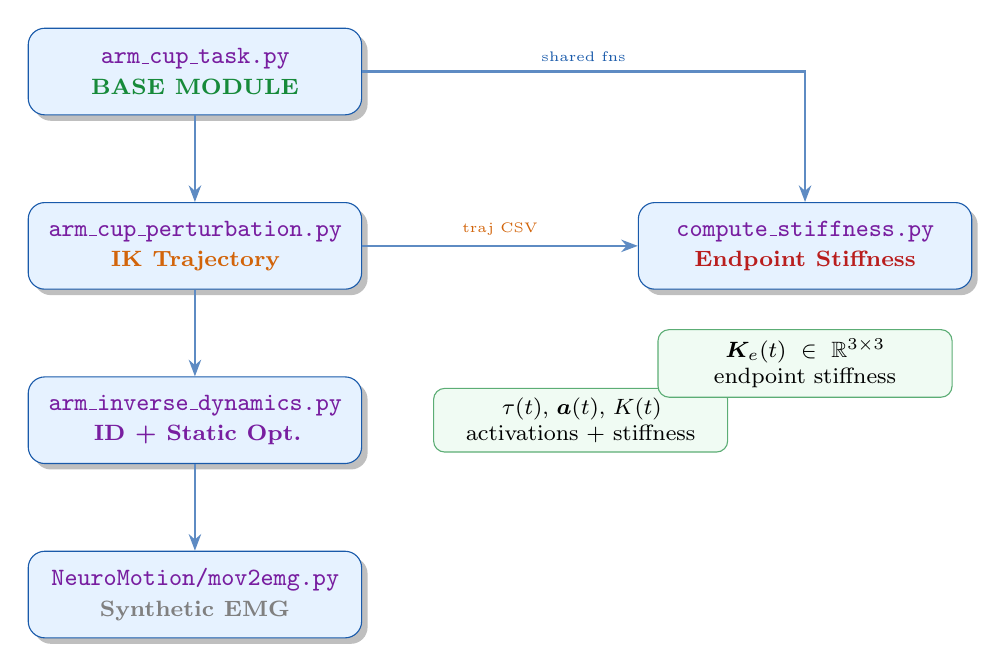
\begin{tikzpicture}[
  node distance = 1.1cm and 2.0cm,
  script/.style = {
    draw=PipeBlue, fill=LightBlue, rounded corners=6pt,
    text width=4.0cm, align=center, font=\small\bfseries,
    minimum height=1.1cm, drop shadow
  },
  outbox/.style = {
    draw=PipeGreen!70, fill=LightGreen!60, rounded corners=4pt,
    text width=3.5cm, align=center, font=\footnotesize,
    minimum height=0.8cm
  },
  arr/.style = {-{Stealth[length=6pt]}, thick, PipeBlue!70}
]
  \node[script] (act) {\file{arm\_cup\_task.py}\\{\footnotesize\color{PipeGreen}BASE MODULE}};
  \node[script, below=of act] (pert) {\file{arm\_cup\_perturbation.py}\\{\footnotesize\color{PipeOrange}IK Trajectory}};
  \node[script, below=of pert] (id)   {\file{arm\_inverse\_dynamics.py}\\{\footnotesize\color{PipePurple}ID + Static Opt.}};
  \node[script, right=3.5cm of pert] (cs) {\file{compute\_stiffness.py}\\{\footnotesize\color{PipeRed}Endpoint Stiffness}};
  \node[script, below=of id]   (nm)   {\file{NeuroMotion/mov2emg.py}\\{\footnotesize\color{gray}Synthetic EMG}};

  \draw[arr] (act)  -- (pert);
  \draw[arr] (pert) -- (id);
  \draw[arr] (id)   -- (nm);
  \draw[arr] (act)  -| node[pos=0.25,above,font=\tiny,PipeBlue]{shared fns} (cs);
  \draw[arr] (pert) -- node[above,font=\tiny,PipeOrange]{traj CSV} (cs);

  \node[outbox, right=0.9cm of id]  {\footnotesize $\tau(t),\,\bm{a}(t),\,K(t)$\\activations + stiffness};
  \node[outbox, below=0.5cm of cs]  {\footnotesize $\bm{K}_e(t) \in \R^{3\times3}$\\endpoint stiffness};
\end{tikzpicture}

\vfill
{\large\bfseries Ball-in-Cup Experimental Platform}\\
{\color{gray} Tele-Impedance / EMG Ground Truth Generation}\\[0.5em]
{\color{gray}\today}
\end{titlepage}

\tableofcontents
\newpage

% ============================================================
\section{Project Overview and Pipeline}
% ============================================================

This document describes the full Python pipeline that generates musculoskeletal
ground-truth data (joint torques, muscle activations, fiber lengths, joint and
endpoint stiffness/damping) for the ball-in-cup reaching task. The data drives
synthetic EMG generation via the NeuroMotion framework and serves as a reference
for learning impedance behaviours in the SEA elbow exosuit controller.

\begin{notebox}[PipeGreen]{Class-based architecture (current)}
Every pipeline script now exposes a single top-level class wrapping its
end-to-end behaviour, and all simulation-wide constants live in a centralised
\file{config.py} (single source of truth). Each class can be driven via
\texttt{ClassName().run()} (replicates the legacy CLI behaviour) or
step-by-step. Backwards compatibility is preserved: every legacy module-level
function (\texttt{build\_trajectory}, \texttt{run\_msk}, \texttt{compute\_moment\_arms},
\texttt{so\_frame}, \dots) remains importable. See
Sec.\,\ref{sec:oo-config} for the full class API and the centralised config map.
\end{notebox}

\subsection{File Dependency Graph}

\begin{center}
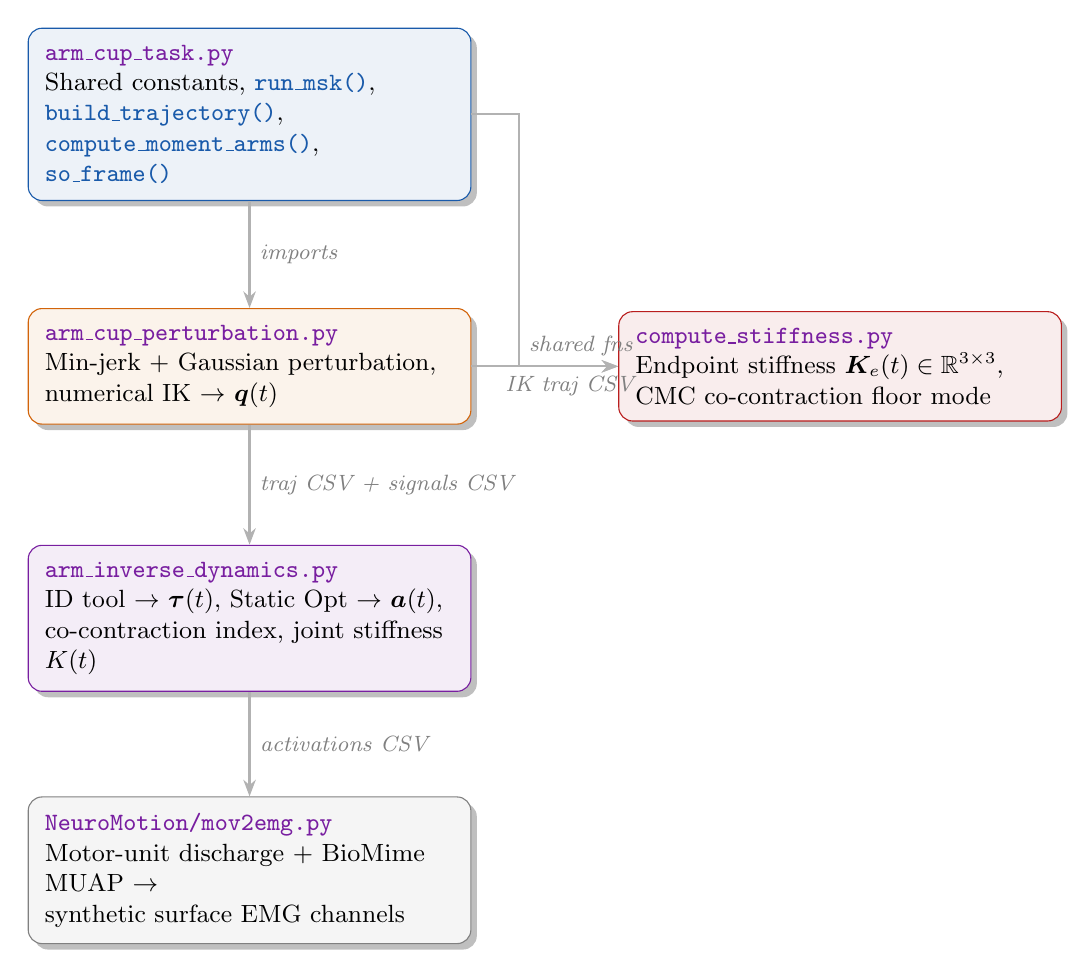
\begin{tikzpicture}[
  box/.style={draw=#1, fill=#1!8, rounded corners=5pt,
              text width=5.2cm, align=left, font=\small,
              inner sep=6pt, drop shadow},
  arr/.style={-{Stealth[length=6pt]}, thick, gray!60},
  lbl/.style={font=\footnotesize\itshape, text=gray}
]
  \node[box=PipeBlue]  (base)  at (0,0)
    {\textbf{\color{PipeBlue}\file{arm\_cup\_task.py}}\\
     \small Shared constants, \py{run\_msk()}, \py{build\_trajectory()},\\
     \py{compute\_moment\_arms()}, \py{so\_frame()}};

  \node[box=PipeOrange] (pert) at (0,-3.2)
    {\textbf{\color{PipeOrange}\file{arm\_cup\_perturbation.py}}\\
     \small Min-jerk + Gaussian perturbation,\\
     numerical IK $\to$ $\bm{q}(t)$};

  \node[box=PipePurple] (id)   at (0,-6.4)
    {\textbf{\color{PipePurple}\file{arm\_inverse\_dynamics.py}}\\
     \small ID tool $\to$ $\bm{\tau}(t)$, Static Opt $\to$ $\bm{a}(t)$,\\
     co-contraction index, joint stiffness $K(t)$};

  \node[box=PipeRed]    (cs)   at (7.5,-3.2)
    {\textbf{\color{PipeRed}\file{compute\_stiffness.py}}\\
     \small Endpoint stiffness $\bm{K}_e(t) \in \R^{3\times3}$,\\
     CMC co-contraction floor mode};

  \node[box=gray]       (nm)   at (0,-9.6)
    {\textbf{\color{gray}\file{NeuroMotion/mov2emg.py}}\\
     \small Motor-unit discharge + BioMime MUAP $\to$\\
     synthetic surface EMG channels};

  \draw[arr] (base)  -- node[lbl,right]{imports} (pert);
  \draw[arr] (pert)  -- node[lbl,right]{traj CSV + signals CSV} (id);
  \draw[arr] (id)    -- node[lbl,right]{activations CSV} (nm);
  \draw[arr] (base.east) -- ++(0.6,0) |- node[lbl,above right]{shared fns} (cs.west);
  \draw[arr] (pert.east) -- ++(0.3,0) |- node[lbl,below right]{IK traj CSV} (cs.west);
\end{tikzpicture}
\end{center}

\subsection{Output Directory Layout}

\begin{tabular}{lll}
\toprule
\textbf{Script} & \textbf{Class} & \textbf{Output subdirectory} \\
\midrule
\rowcolor{LightBlue}   \file{arm\_cup\_task.py}          & \py{ArmCupTask}           & \outdir{demo\_output/arm\_cup\_task/} \\
\rowcolor{LightOrange} \file{arm\_cup\_perturbation.py}  & \py{ArmCupPerturbation}   & \outdir{demo\_output/arm\_cup\_perturbation/} \\
\rowcolor{LightPurple} \file{arm\_inverse\_dynamics.py}  & \py{ArmInverseDynamics}   & \outdir{demo\_output/arm\_inverse\_dynamics/} \\
\rowcolor{LightRed}    \file{compute\_stiffness.py}      & \py{ComputeStiffness}     & \outdir{demo\_output/compute\_stiffness/} \\
\rowcolor{LightGreen}  \file{compare\_to\_razavian2021.py}& \py{RazavianComparison}   & \outdir{demo\_output/compare\_razavian/} \\
\bottomrule
\end{tabular}

\medskip
All constants are imported from \file{config.py}; no script redeclares
shared values locally.

\subsection{Execution Sequence}

Each script can be invoked from the command line (legacy entry point) or
driven programmatically through its public class.

\begin{codebox}{Run order — CLI}
# Step 1 -- IK-solved trajectory with mechanical perturbation
python arm_cup_perturbation.py

# Step 2 -- Inverse dynamics + static optimisation + joint stiffness
python arm_inverse_dynamics.py

# Step 3 -- Endpoint stiffness K_e(t) and damping D_e(t)
python compute_stiffness.py --mode perturb --stiffness static_opt
# or with CMC co-contraction floor:
python compute_stiffness.py --mode perturb --stiffness cmc

# Step 4 -- Quantitative comparison vs. Razavian et al. ICRA 2021
python compare_to_razavian2021.py
\end{codebox}

\begin{codebox}{Run order — Class API (equivalent)}
from arm_cup_perturbation    import ArmCupPerturbation
from arm_inverse_dynamics    import ArmInverseDynamics
from compute_stiffness       import ComputeStiffness
from compare_to_razavian2021 import RazavianComparison

ArmCupPerturbation().run()                                       # Step 1
ArmInverseDynamics(tag="perturb").run()                          # Step 2
ComputeStiffness(mode="perturb", stiffness="cmc").run()          # Step 3
RazavianComparison().run()                                       # Step 4
\end{codebox}

\subsection{Notation and Symbol Table}

The following symbols are used consistently throughout all four scripts and this document.
$m\in\{1\ldots14\}$ indexes muscles; $i\in\{x,y,z\}$ indexes Cartesian components;
$j$ or $k$ indexes generalised coordinates.
$n_\text{dof}\in\{2,7\}$ depending on context:
\file{arm\_inverse\_dynamics.py} operates on the 2 IK-active DOFs;
\file{compute\_stiffness.py} uses all 7 active DOFs.

\begin{center}
\small
\begin{tabular}{llll}
\toprule
\textbf{Symbol} & \textbf{Shape} & \textbf{Description} & \textbf{Units} \\
\midrule
\rowcolor{LightBlue}
$\bq(t)$ & $\R^7$ & Generalised joint coordinate vector & rad \\
$\dot{\bq}(t)$ & $\R^7$ & Joint angular velocities & rad/s \\
\rowcolor{LightBlue}
$\ddot{\bq}(t)$ & $\R^7$ & Joint angular accelerations & rad/s$^2$ \\
$\btau(t)$ & $\R^{n_\text{dof}}$ & Generalised joint torques (output of ID) & N$\cdot$m \\
\rowcolor{LightBlue}
$\ba(t)$ & $\R^{14}$ & Muscle activation vector (output of SO), $a_m\in[0,1]$ & -- \\
$\bR(t)$ & $\R^{n_\text{dof}\times14}$ & Moment arm matrix: $R_{im}=\partial l_m/\partial q_i$ & m/rad \\
\rowcolor{LightBlue}
$\bF_0$ & $\R^{14}$ & Maximum isometric muscle forces (model constants) & N \\
$\bm{fl}(t)$ & $\R^{14}$ & Active force--length multiplier per muscle & -- \\
\rowcolor{LightBlue}
$l_m(t)$ & scalar & Current fiber length of muscle $m$ & m \\
$L_{\text{opt},m}$ & scalar & Optimal fiber length of muscle $m$ (model const.) & m \\
\rowcolor{LightBlue}
$\tilde{l}_m = l_m/L_\text{opt}$ & scalar & Normalised fiber length ($=1$ at peak force) & -- \\
$k_m(t)$ & scalar & Linearised muscle stiffness (Hill model) & N/m \\
\rowcolor{LightBlue}
$\bJ(t)$ & $\R^{3\times n_\text{dof}}$ & Hand endpoint Jacobian: $J_{ij}=\partial p_i/\partial q_j$ & m/rad \\
$\bJ^+$ & $\R^{n_\text{dof}\times3}$ & Moore--Penrose pseudoinverse of $\bJ$ & rad/m \\
\rowcolor{LightBlue}
$\bK_\text{joint}(t)$ & $\R^{n_\text{dof}\times n_\text{dof}}$ & Joint stiffness tensor & N$\cdot$m/rad \\
$\bm{K}_e(t)$ & $\R^{3\times3}$ & Cartesian endpoint stiffness tensor & N/m \\
\rowcolor{LightBlue}
$\bm{D}_e(t)$ & $\R^{3\times3}$ & Cartesian endpoint damping tensor & N$\cdot$s/m \\
$d_m(t)$ & scalar & Hill linearised muscle damping (per muscle) & N$\cdot$s/m \\
\rowcolor{LightBlue}
$\beta_D$ & 0.3 & Hill f-v slope coefficient near $v_m=0$ (Zajac 1989) & -- \\
$V_\text{max,factor}$ & 10 s$^{-1}$ & $v_\text{max}=V_\text{max,factor}\cdot l_\text{opt}$ & 1/s \\
\rowcolor{LightBlue}
$\lambda_{\min},\,\lambda_{\max}$ & scalar & Eigenvalues of $\bm{K}_e[0:2,0:2]$ (XY sub-block) & N/m \\
$P_\text{null}(t)$ & scalar & Null-space co-contraction proxy: $\min_m a_m$ & -- \\
\rowcolor{LightBlue}
$c_\text{exo}(t)$ & scalar & SEA exo-cable pre-tension setpoint (driven by $P_\text{null}$) & m \\
$F_\text{int}(t)$ & scalar & Interaction force at hand--cup interface & N \\
\rowcolor{LightBlue}
$\hat{\bm{d}}$ & $\R^3$ & Unit direction of hand motion (ground frame) & -- \\
$\beta$ & 40 & Hill stiffness dimensionless scaling coefficient (\file{arm\_inverse\_dynamics.py} only) & -- \\
\rowcolor{LightBlue}
$\gamma$ & 0.45 & Gaussian force--length curve width parameter & -- \\
$\alpha_\text{floor}$ & 0.15 (CMC) & SLSQP lower bound on all activations in perturbation window & -- \\
\rowcolor{LightBlue}
$M_\text{eff}$ & 2.0 kg & Effective inertial mass of cup + ball & kg \\
$D$ & 0.30 m & Reach distance along the rail & m \\
\rowcolor{LightBlue}
$T$ & 1.60 s & Reach duration & s \\
$T_\text{pert}$ & 0.90 s & Centre of Gaussian perturbation & s \\
\rowcolor{LightBlue}
$\sigma$ & 0.030 s & Width (std dev) of Gaussian perturbation & s \\
$\tau = t/T$ & scalar & Normalised time within a movement segment, $\tau\in[0,1]$ & -- \\
\bottomrule
\end{tabular}
\end{center}


% ============================================================
\section{Detailed Block Diagram — ID and ComputeStiffness}
\label{sec:block-diagram}
% ============================================================

This section gives a per-block view of \file{arm\_inverse\_dynamics.py}
(\py{ArmInverseDynamics}) and \file{compute\_stiffness.py}
(\py{ComputeStiffness}). Each block lists \textbf{(a)} what it consumes,
\textbf{(b)} the formula it implements, and \textbf{(c)} what it produces.

% ----------------------------------------------------------------
\subsection{\texttt{ArmInverseDynamics} — Block Diagram}
% ----------------------------------------------------------------

\begin{center}
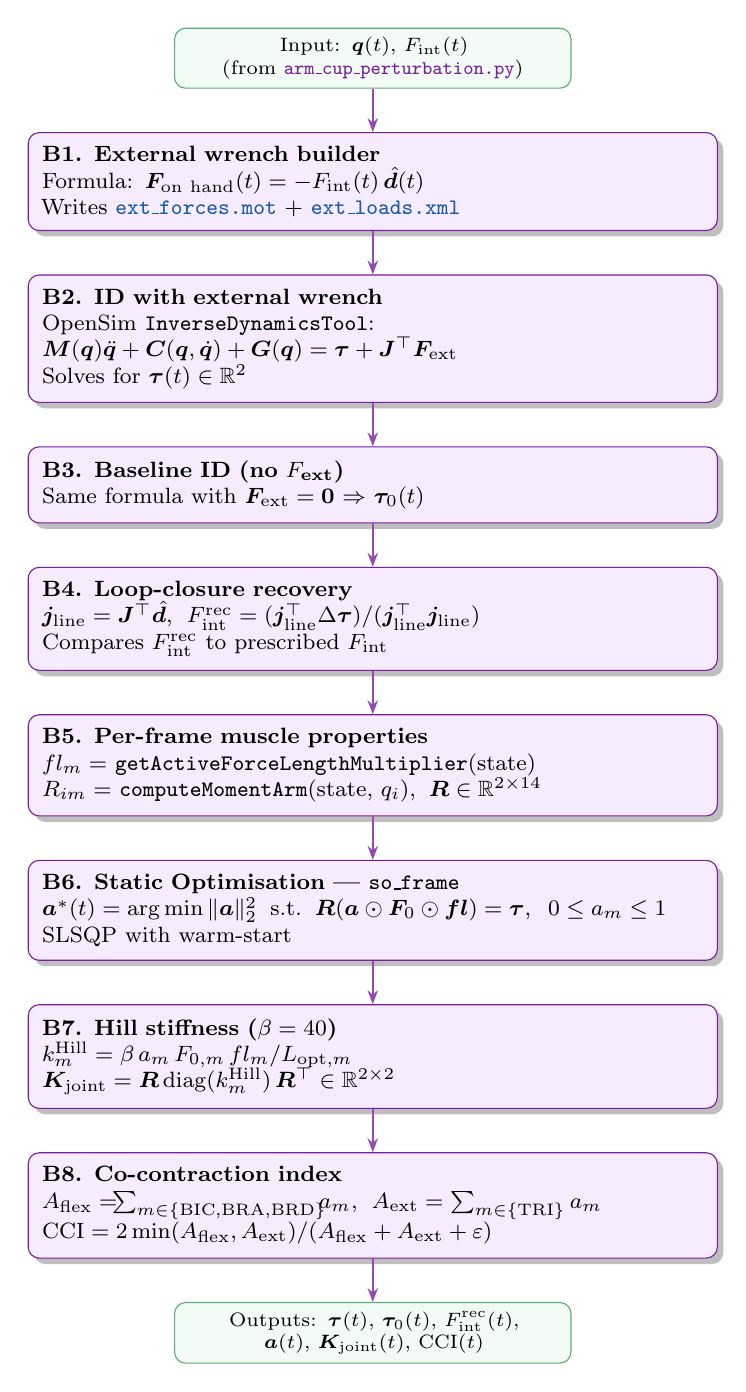
\begin{tikzpicture}[
  node distance=0.55cm and 1.0cm,
  blk/.style ={draw=PipePurple, fill=LightPurple, rounded corners=4pt,
               text width=8.4cm, align=left, font=\footnotesize,
               inner sep=5pt, minimum height=0.9cm, drop shadow},
  data/.style={draw=PipeGreen!70, fill=LightGreen!50, rounded corners=4pt,
               text width=4.8cm, align=center, font=\scriptsize,
               minimum height=0.6cm},
  arr/.style ={-{Stealth[length=5pt]}, thick, PipePurple!80}
]
  \node[data] (in) {Input: $\bq(t)$, $F_\text{int}(t)$\\(from \file{arm\_cup\_perturbation.py})};

  \node[blk, below=of in] (b1)
   {\textbf{B1. External wrench builder}\\
    Formula: $\bF_\text{on hand}(t) = -F_\text{int}(t)\,\hat{\bm{d}}(t)$\\
    Writes \py{ext\_forces.mot} + \py{ext\_loads.xml}};
  \node[blk, below=of b1] (b2)
   {\textbf{B2. ID with external wrench}\\
    OpenSim \texttt{InverseDynamicsTool}:\\
    $\bm{M}(\bq)\ddot{\bq}+\bm{C}(\bq,\dot{\bq})+\bm{G}(\bq)=\btau+\bJ^\top\bF_\text{ext}$\\
    Solves for $\btau(t)\in\R^2$};
  \node[blk, below=of b2] (b3)
   {\textbf{B3. Baseline ID (no $F_\text{ext}$)}\\
    Same formula with $\bF_\text{ext}=\bm{0}$ $\Rightarrow$ $\btau_0(t)$};
  \node[blk, below=of b3] (b4)
   {\textbf{B4. Loop-closure recovery}\\
    $\bm{j}_\text{line}=\bJ^\top\hat{\bm{d}}$,\;
    $F^{\text{rec}}_\text{int}=(\bm{j}_\text{line}^\top\Delta\btau)/(\bm{j}_\text{line}^\top\bm{j}_\text{line})$\\
    Compares $F^{\text{rec}}_\text{int}$ to prescribed $F_\text{int}$};
  \node[blk, below=of b4] (b5)
   {\textbf{B5. Per-frame muscle properties}\\
    $fl_m=$ \texttt{getActiveForceLengthMultiplier}(state)\\
    $R_{im}=$ \texttt{computeMomentArm}(state, $q_i$),\;\;$\bR\in\R^{2\times14}$};
  \node[blk, below=of b5] (b6)
   {\textbf{B6. Static Optimisation — \texttt{so\_frame}}\\
    $\ba^*(t)=\arg\min\|\ba\|_2^2$\;\;s.t.\;\;$\bR(\ba\odot\bF_0\odot\bm{fl})=\btau,\;\;0\le a_m\le 1$\\
    SLSQP with warm-start};
  \node[blk, below=of b6] (b7)
   {\textbf{B7. Hill stiffness ($\beta=40$)}\\
    $k_m^\text{Hill}=\beta\,a_m\,F_{0,m}\,fl_m/L_{\text{opt},m}$\\
    $\bK_\text{joint}=\bR\,\mathrm{diag}(k_m^\text{Hill})\,\bR^\top\in\R^{2\times2}$};
  \node[blk, below=of b7] (b8)
   {\textbf{B8. Co-contraction index}\\
    $A_\text{flex}=\!\!\!\sum_{m\in\{\text{BIC,BRA,BRD}\}}\!\!\!a_m$,\;
    $A_\text{ext}=\sum_{m\in\{\text{TRI}\}}a_m$\\
    $\text{CCI}=2\min(A_\text{flex},A_\text{ext})/(A_\text{flex}+A_\text{ext}+\varepsilon)$};

  \node[data, below=of b8] (out)
   {Outputs: $\btau(t)$, $\btau_0(t)$, $F^{\text{rec}}_\text{int}(t)$,\\
    $\ba(t)$, $\bK_\text{joint}(t)$, $\text{CCI}(t)$};

  \draw[arr] (in) -- (b1);  \draw[arr] (b1) -- (b2);
  \draw[arr] (b2) -- (b3);  \draw[arr] (b3) -- (b4);
  \draw[arr] (b4) -- (b5);  \draw[arr] (b5) -- (b6);
  \draw[arr] (b6) -- (b7);  \draw[arr] (b7) -- (b8);
  \draw[arr] (b8) -- (out);
\end{tikzpicture}
\end{center}

% ----------------------------------------------------------------
\subsection{\texttt{ComputeStiffness} — Block Diagram}
% ----------------------------------------------------------------

\begin{center}
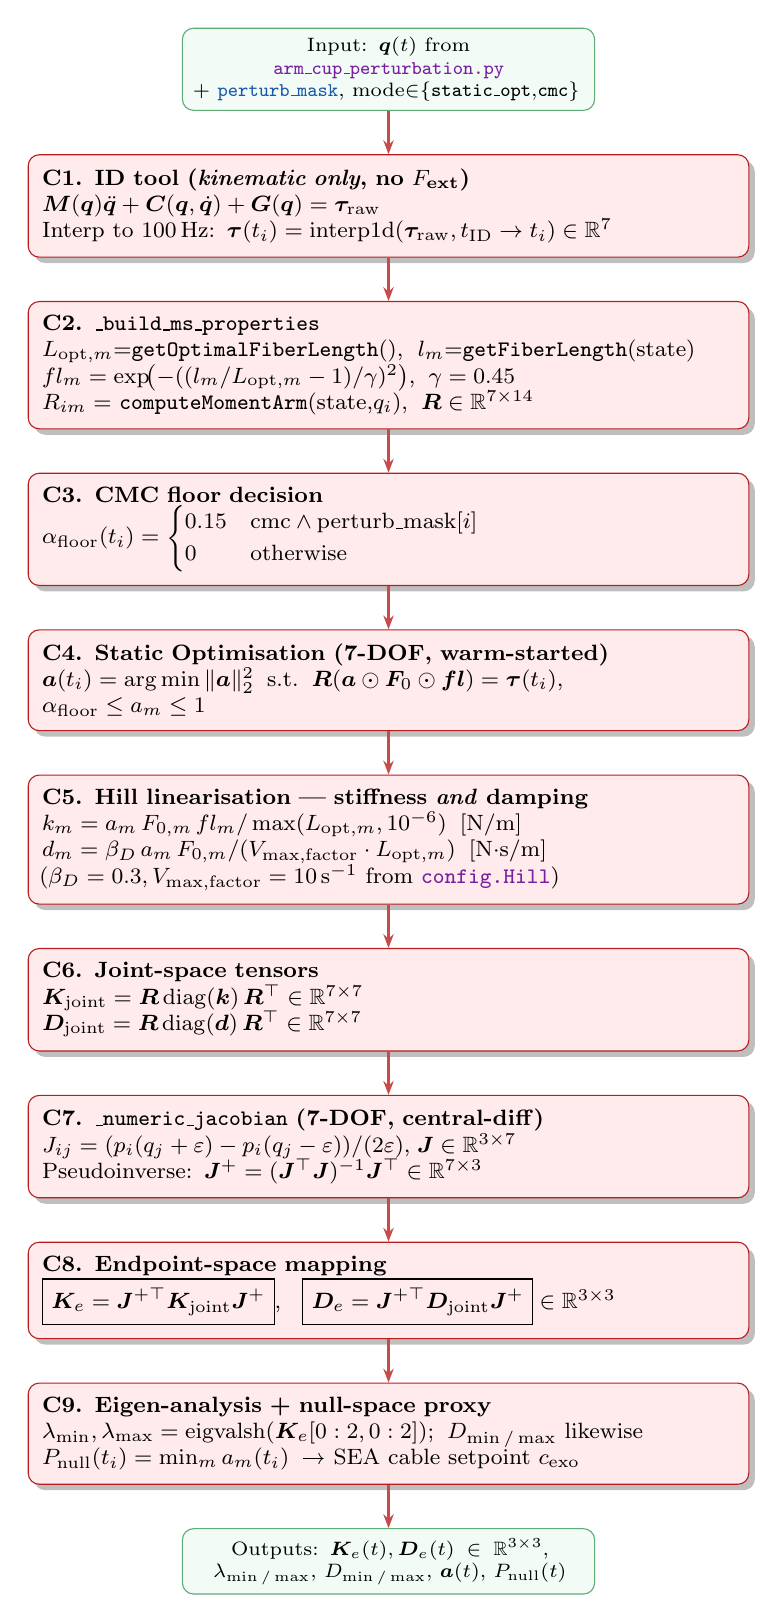
\begin{tikzpicture}[
  node distance=0.55cm and 1.0cm,
  blk/.style ={draw=PipeRed, fill=LightRed, rounded corners=4pt,
               text width=8.8cm, align=left, font=\footnotesize,
               inner sep=5pt, minimum height=0.9cm, drop shadow},
  data/.style={draw=PipeGreen!70, fill=LightGreen!50, rounded corners=4pt,
               text width=5.0cm, align=center, font=\scriptsize,
               minimum height=0.6cm},
  arr/.style ={-{Stealth[length=5pt]}, thick, PipeRed!80}
]
  \node[data] (in)
   {Input: $\bq(t)$ from \file{arm\_cup\_perturbation.py}\\
    + \py{perturb\_mask}, mode$\in$\{\texttt{static\_opt},\texttt{cmc}\}};

  \node[blk, below=of in] (c1)
   {\textbf{C1. ID tool (\emph{kinematic only}, no $F_\text{ext}$)}\\
    $\bm{M}(\bq)\ddot{\bq}+\bm{C}(\bq,\dot{\bq})+\bm{G}(\bq)=\btau_\text{raw}$\\
    Interp to 100\,Hz: $\btau(t_i)=\text{interp1d}(\btau_\text{raw}, t_\text{ID}\to t_i)\in\R^7$};
  \node[blk, below=of c1] (c2)
   {\textbf{C2. \texttt{\_build\_ms\_properties}}\\
    $L_{\text{opt},m}$=\texttt{getOptimalFiberLength}(),\;
    $l_m$=\texttt{getFiberLength}(state)\\
    $fl_m=\exp\!\bigl(-((l_m/L_{\text{opt},m}-1)/\gamma)^2\bigr)$,\;\;$\gamma=0.45$\\
    $R_{im}=$ \texttt{computeMomentArm}(state,$q_i$),\;\;$\bR\in\R^{7\times14}$};
  \node[blk, below=of c2] (c3)
   {\textbf{C3. CMC floor decision}\\
    $\alpha_\text{floor}(t_i)=\begin{cases}0.15 & \text{cmc}\wedge\text{perturb\_mask}[i]\\ 0 & \text{otherwise}\end{cases}$};
  \node[blk, below=of c3] (c4)
   {\textbf{C4. Static Optimisation (7-DOF, warm-started)}\\
    $\ba(t_i)=\arg\min\|\ba\|_2^2$\;\;s.t.\;\;$\bR(\ba\odot\bF_0\odot\bm{fl})=\btau(t_i)$,\\
    $\alpha_\text{floor}\le a_m\le 1$};
  \node[blk, below=of c4] (c5)
   {\textbf{C5. Hill linearisation — stiffness \emph{and} damping}\\
    $k_m=a_m\,F_{0,m}\,fl_m/\max(L_{\text{opt},m},10^{-6})$\;\;[N/m]\\
    $d_m=\beta_D\,a_m\,F_{0,m}/(V_\text{max,factor}\cdot L_{\text{opt},m})$\;\;[N$\cdot$s/m]\\
    ($\beta_D=0.3$,\,$V_\text{max,factor}=10$\,s$^{-1}$ from \file{config.Hill})};
  \node[blk, below=of c5] (c6)
   {\textbf{C6. Joint-space tensors}\\
    $\bK_\text{joint}=\bR\,\mathrm{diag}(\bm{k})\,\bR^\top\in\R^{7\times7}$\\
    $\bD_\text{joint}=\bR\,\mathrm{diag}(\bm{d})\,\bR^\top\in\R^{7\times7}$};
  \node[blk, below=of c6] (c7)
   {\textbf{C7. \texttt{\_numeric\_jacobian} (7-DOF, central-diff)}\\
    $J_{ij}=(p_i(q_j+\varepsilon)-p_i(q_j-\varepsilon))/(2\varepsilon)$,\;$\bJ\in\R^{3\times7}$\\
    Pseudoinverse: $\bJ^+=(\bJ^\top\bJ)^{-1}\bJ^\top\in\R^{7\times3}$};
  \node[blk, below=of c7] (c8)
   {\textbf{C8. Endpoint-space mapping}\\
    $\boxed{\bm{K}_e=\bJ^{+\top}\bK_\text{joint}\bJ^+}$,\;\;
    $\boxed{\bm{D}_e=\bJ^{+\top}\bD_\text{joint}\bJ^+}\in\R^{3\times3}$};
  \node[blk, below=of c8] (c9)
   {\textbf{C9. Eigen-analysis + null-space proxy}\\
    $\lambda_{\min},\lambda_{\max}=\mathrm{eigvalsh}(\bm{K}_e[0:2,0:2])$;\;\;$D_{\min/\max}$ likewise\\
    $P_\text{null}(t_i)=\min_m a_m(t_i)$\;\;→ SEA cable setpoint $c_\text{exo}$};

  \node[data, below=of c9] (out)
   {Outputs: $\bm{K}_e(t),\bm{D}_e(t)\in\R^{3\times3}$,\\
    $\lambda_{\min/\max}$, $D_{\min/\max}$, $\ba(t)$, $P_\text{null}(t)$};

  \draw[arr] (in) -- (c1);  \draw[arr] (c1) -- (c2);
  \draw[arr] (c2) -- (c3);  \draw[arr] (c3) -- (c4);
  \draw[arr] (c4) -- (c5);  \draw[arr] (c5) -- (c6);
  \draw[arr] (c6) -- (c7);  \draw[arr] (c7) -- (c8);
  \draw[arr] (c8) -- (c9);  \draw[arr] (c9) -- (out);
\end{tikzpicture}
\end{center}

\begin{notebox}[PipeOrange]{Why \py{ArmInverseDynamics} and \py{ComputeStiffness} differ}
\begin{itemize}\itemsep2pt
  \item \textbf{B2 vs.\ C1}: B2 passes \texttt{ExternalLoads} XML to the ID
    tool, so $\btau$ \emph{includes} the cup-rail $F_\text{int}$ spike.
    C1 omits the wrench, so $\btau$ represents free-reaching demand only.
  \item \textbf{Active DOFs}: B5--B8 use $n_\text{dof}=2$ (elv\_angle,
    elbow\_flexion); C2--C9 use $n_\text{dof}=7$ (all active DOFs).
  \item \textbf{Hill scale}: B7 uses $\beta=40$ (large joint stiffness numbers);
    C5 uses $\beta=1$ (raw Hill linearisation). Qualitative $\bm{K}_e$
    modulation is identical; absolute magnitude differs by $\sim 40\times$.
  \item \textbf{Damping}: only \py{ComputeStiffness} computes $\bm{D}_e(t)$
    via the Hill f-v slope ($d_m=\beta_D a_m F_0/(V_\text{max,factor}L_\text{opt})$).
  \item \textbf{CMC mode}: \py{ComputeStiffness} compensates for the missing
    $F_\text{int}$ by raising $\alpha_\text{floor}=0.15$ during the
    perturbation window, injecting null-space stiffening that mirrors what
    \py{ArmInverseDynamics} captures naturally through the $\btau$ spike.
\end{itemize}
\end{notebox}


% ============================================================
\section{\texttt{arm\_cup\_task.py} — Base Module}
% ============================================================

\file{arm\_cup\_task.py} is the shared hub. Every other script imports
constants, helper functions, and now the Static Optimisation primitives
from it.  It is also runnable standalone to generate a pure sinusoidal
or min-jerk trajectory with passive fiber lengths.

\subsection{Shared Constants}

\begin{tabular}{lll}
\toprule
\textbf{Constant} & \textbf{Value} & \textbf{Description} \\
\midrule
\rowcolor{gray!6} \py{FS}          & 100 Hz       & Kinematic sample rate \\
\py{MS\_LABELS}   & 14 muscles    & Surface-EMG relevant subset \\
\rowcolor{gray!6} \py{ACTIVE\_DOFS} & 7 DOFs      & MoBL-ARMS active coordinates \\
\py{NEUTRAL}      & (see below)   & Reference hold posture (radians) \\
\rowcolor{gray!6} \py{MODEL\_PATH} & \texttt{model/MOBL\_ARMS\_41.osim} & OpenSim model \\
\bottomrule
\end{tabular}

\medskip
\textbf{Neutral posture} (degrees):
\hspace{1em}$\varphi_\text{elv} = 52.9^\circ$,\;
$\varphi_\text{sev} = 80.4^\circ$,\;
$\varphi_\text{srot} = 58.0^\circ$,\;
$\varphi_\text{ef} = 65.6^\circ$,\;
$\varphi_\text{ps} = -0.9^\circ$

\subsection{Trajectory Builders}

\subsubsection{Sinusoidal (Lissajous) mode}

\begin{eqbox}{Sine trajectory — \texttt{build\_trajectory\_sine()}}
\begin{equation}
q_i(t) = q_i^{0} + A_i \sin(2\pi f t + \phi_i),
\qquad f = 0.5\,\text{Hz},\quad t \in [0, 8]\,\text{s}
\end{equation}
where $A_{\text{shoulder\_rot}}=15^\circ$, $A_{\text{shoulder\_elv}}=10^\circ$,
$\phi_{\text{shoulder\_rot}}=\pi/2$
(90$^\circ$ phase produces a circular Lissajous path on the 2-D rail).
\end{eqbox}

\subsubsection{Minimum-jerk (waypoint) mode}

\begin{eqbox}{Min-jerk trajectory — \texttt{build\_trajectory\_min\_jerk()}}
Between consecutive waypoints separated by duration $T$, each DOF follows:
\begin{equation}
q_i(t) = q_i^{\text{start}}
  + \bigl(q_i^{\text{end}} - q_i^{\text{start}}\bigr)
    \underbrace{\!\left(10\tau^3 - 15\tau^4 + 6\tau^5\right)\!}_{s(\tau)},
\quad \tau = t/T \in [0,1]
\end{equation}
This minimises the integral of squared jerk $\int_0^T \dddot{q}^2\,\mathrm{d}t$
(Flash \& Hogan 1985), producing the characteristic bell-shaped velocity profile.
\end{eqbox}

\begin{notebox}[PipeBlue]{Numerical example --- min-jerk position and velocity}
Parameters: $D=0.30\,\text{m}$, $T=1.60\,\text{s}$; DOF example:
\dof{elv\_angle} moves from $q_\text{start}=52.9^\circ$ to $q_\text{end}=62.5^\circ$.
At $t=0.80\,\text{s}$ ($\tau=0.80/1.60=0.500$):
\begin{align*}
s(0.5) &= 10(0.5)^3 - 15(0.5)^4 + 6(0.5)^5
        = 1.250 - 0.938 + 0.188 = \mathbf{0.500}
        \qquad(\text{half of range traversed})\\[4pt]
q_\text{elv}(0.8\,\text{s}) &= 52.9^\circ + (62.5-52.9)^\circ\times0.500
        = 52.9^\circ + 4.8^\circ = \mathbf{57.7^\circ}\\[4pt]
\dot{x}_\text{mj}(0.8\,\text{s})
  &= \tfrac{0.30}{1.60}\bigl(30(0.25)-60(0.125)+30(0.0625)\bigr)
   = 0.1875\times1.875 = \mathbf{0.352\,\text{m/s}} \;\text{(peak cup speed)}
\end{align*}
The peak cup velocity $0.352\,\text{m/s}$ occurs precisely at $\tau=0.5$.
The velocity profile is symmetric and bell-shaped: it starts and ends at
zero, with no discontinuities in acceleration or jerk at the endpoints.
\end{notebox}

\subsection{Shared Static Optimisation Primitives}

\subsubsection{\texttt{compute\_moment\_arms}}

\begin{eqbox}{\texttt{compute\_moment\_arms(model, state, ms\_labels, dofs)}}
Returns $\bR \in \R^{n_\text{dof} \times n_\text{ms}}$ where
\begin{equation}
R_{ij} = \frac{\partial l_{\text{m},j}}{\partial q_i}
       = \texttt{muscle}_j\texttt{.computeMomentArm(state, coord}_i\texttt{)}
\end{equation}
Requires state $\geq$ \texttt{Position}-realised.
\end{eqbox}

\subsubsection{\texttt{so\_frame} — Per-frame Static Optimisation}

\begin{eqbox}{\texttt{so\_frame($\btau$, $\bR$, $\bF_0$, $\bm{fl}$, alpha\_floor, x0)}}
\begin{equation}
\min_{\ba} \;\|\ba\|_2^2 \qquad
\text{s.t.}\quad \bR\,(\ba \odot \bF_0 \odot \bm{fl}) = \btau,
\quad \alpha_\text{floor} \leq a_j \leq 1
\end{equation}
Solved with SciPy SLSQP (\texttt{ftol=1e-8}, \texttt{maxiter=400}).
\begin{itemize}\itemsep0pt
  \item $\bm{fl} \in \R^{n_\text{ms}}$: active force--length multiplier per muscle
  \item $\bF_0 \in \R^{n_\text{ms}}$: maximum isometric force per muscle
  \item \texttt{alpha\_floor $>$ 0}: CMC co-contraction mode (null-space stiffening)
  \item \texttt{x0}: warm-start from previous frame (improves convergence)
\end{itemize}
\end{eqbox}

\begin{notebox}[PipeBlue]{Numerical example --- 2-muscle SO (one elbow DOF)}
One frame, $\tau_\text{ef}=5.0\,\text{N}{\cdot}\text{m}$ (net flexion), two muscles:
\begin{center}\small
\begin{tabular}{lllll}
\toprule
Muscle & $F_{0,m}$ & $fl_m$ & $R_{m,\text{ef}}$ & $R_{m}F_{0,m}fl_m$~per unit $a_m$ \\
\midrule
BIClong & 629\,N & 0.85 & $+0.045$\,m & $+24.06$\,N$\cdot$m \\
TRIlong & 798\,N & 0.70 & $-0.025$\,m & $-13.97$\,N$\cdot$m \\
\bottomrule
\end{tabular}
\end{center}
Equality constraint:
$24.06\,a_\text{BIC} - 13.97\,a_\text{TRI} = 5.0$; \quad
minimum-norm solution ($a_\text{TRI}=0$, pure flexion):
\[
a_\text{BIC}^* = 5.0/24.06 = \mathbf{0.208}, \qquad a_\text{TRI}^*=\mathbf{0},
\qquad \|\ba\|_2^2 = 0.0433
\]
\textbf{CMC co-contraction case} ($\alpha_\text{floor}=0.15$):
both muscles are forced $\geq0.15$.
SLSQP sets $a_\text{TRI}=0.15$, then $a_\text{BIC}=(5.0+13.97\times0.15)/24.06=0.295$.
\[
\|\ba\|_2^2 = 0.295^2 + 0.15^2 = 0.0870 + 0.0225 = \mathbf{0.110}
\quad (\text{2.5}\times\text{ higher effort; all }k_m\text{ rise similarly})
\]
\end{notebox}


% ============================================================
\section{\texttt{arm\_cup\_perturbation.py} — IK Trajectory}
% ============================================================

Generates a point-to-point reaching motion (left $\to$ right along a
horizontal line) with a single mechanical perturbation modelling a
ball-disturbance event.  Two active DOFs are IK-solved; five are locked.

\subsection{Locked and Active DOFs}

\begin{tabular}{lll}
\toprule
\textbf{DOF} & \textbf{Role} & \textbf{Value} \\
\midrule
\rowcolor{gray!6}\dof{shoulder\_elv} & Locked & $80.4^\circ$ (neutral) \\
\dof{shoulder\_rot} & Locked & $58.0^\circ$ (neutral) \\
\rowcolor{gray!6}\dof{pro\_sup}      & Locked & $-0.9^\circ$ (neutral) \\
\dof{deviation}     & Locked & $0.1^\circ$ (neutral) \\
\rowcolor{gray!6}\dof{flexion}       & Locked & $-0.3^\circ$ (neutral) \\
\midrule
\dof{elv\_angle}     & \textbf{IK-solved} & varies \\
\rowcolor{gray!6}\dof{elbow\_flexion} & \textbf{IK-solved} & varies \\
\bottomrule
\end{tabular}

\subsection{1-D Trajectory: Min-Jerk + Gaussian Perturbation}

\begin{eqbox}{Prescribed velocity and interaction force}
\textbf{Baseline velocity} (min-jerk):
\begin{equation}
\dot{x}_\text{mj}(t) = \frac{D}{T}\Bigl(30\tau^2 - 60\tau^3 + 30\tau^4\Bigr),
\quad \tau = t/T
\end{equation}

\textbf{Velocity dip} (braking perturbation):
\begin{equation}
\dot{x}(t) = \dot{x}_\text{mj}(t) - \underbrace{\alpha_v \cdot \dot{x}_\text{mj}(T_\text{pert})
\cdot \exp\!\left(-\tfrac{(t-T_\text{pert})^2}{2\sigma^2}\right)}_{\text{Gaussian dip}}
\end{equation}

\textbf{Interaction force} (three-component purple-line model):
\begin{equation}
F_\text{int}(t) = \underbrace{M_\text{eff}\,\ddot{x}_\text{mj}(t)}_{\text{inertial baseline}}
  + \underbrace{F_\text{spike}\exp\!\left(-\tfrac{(t-T_\text{pert})^2}{2\sigma^2}\right)}_{\text{perturbation spike}}
  - \underbrace{F_\text{neg}\exp\!\left(-\tfrac{(t-T_\text{pert}-\Delta t)^2}{2\sigma_\text{neg}^2}\right)}_{\text{post-spike undershoot}}
\end{equation}
Default parameters: $D=0.30\,\text{m}$, $T=1.60\,\text{s}$,
$T_\text{pert}=0.90\,\text{s}$, $\sigma=0.030\,\text{s}$,
$F_\text{spike}=12\,\text{N}$, $M_\text{eff}=2.0\,\text{kg}$.
\end{eqbox}

\begin{notebox}[PipeBlue]{Numerical example --- $F_\text{int}$ at perturbation peak ($t=0.90\,\text{s}$)}
$\tau=0.90/1.60=0.5625$, so $\tau^2=0.3164$, $\tau^3=0.1781$.
\begin{align*}
\ddot{x}_\text{mj}(0.9) &= \frac{D}{T^2}(60\tau-180\tau^2+120\tau^3)
  = \frac{0.30}{2.56}(33.75-56.95+21.37)\\
  &= 0.1172\times(-1.83) = -0.215\,\text{m/s}^2
  \quad(\text{cup decelerating near target})
\end{align*}
Three-component breakdown at $t=T_\text{pert}$ (Gaussian exponent $=0$):
\[
F_\text{inertial}= 2.0\times(-0.215)=-0.43\,\text{N},\quad
F_\text{spike}\,e^{0}=12.0\,\text{N},\quad
F_\text{neg}\approx0\;\text{(zero at peak)}
\]
\[
\Rightarrow\quad F_\text{int}(0.90\,\text{s})\approx -0.43+12.0 \approx \mathbf{11.6\,\text{N}}
\]
The inertial term is small at the perturbation centre because the cup velocity is near-peak
(acceleration is small). The $12\,\text{N}$ spike dominates. The post-spike undershoot
(negative lobe, delayed by $\Delta t$) models the restoring force as the ball settles
back, but is negligible at $t=T_\text{pert}$ itself.
\end{notebox}

\subsection{Numerical IK}

\begin{eqbox}{Inverse Kinematics — \texttt{\_solve\_ik()}}
The 1-D cup position $x(t)$ maps to a 3-D hand target along the
pre-computed line:
\begin{equation}
\bm{p}_\text{target}(t) = \bm{c} + x(t)\,\hat{\bm{d}}
\end{equation}
where $\bm{c}$ is the line centre (FK at neutral) and $\hat{\bm{d}}$ is
the unit direction.  At each of the $N_\text{IK}=20\,\text{Hz}$ coarse
frames, the joint angles are found by:
\begin{equation}
\bm{q}_{\text{IK}}^* = \arg\min_{\bm{q}}
  \left\|\text{FK}(\bm{q}) - \bm{p}_\text{target}\right\|_2^2
\end{equation}
solved with L-BFGS-B, then cubic-spline interpolated to 100\,Hz.
\end{eqbox}

\begin{notebox}[PipeOrange]{Output files — \outdir{demo\_output/arm\_cup\_perturbation/}}
\begin{tabular}{ll}
\py{cup\_task\_trajectory\_perturb.csv} & All 7 DOFs at 100\,Hz \\
\py{cup\_task\_signals\_perturb.csv}    & $t, x, \dot{x}, \ddot{x}, F_\text{pert}, F_\text{int}$ \\
\py{cup\_task\_trajectory\_perturb.mot} & OpenSim motion file \\
\end{tabular}
\end{notebox}

\subsection{Output Plots}

\begin{figure}[H]
\centering
\begin{subfigure}[t]{0.48\textwidth}
  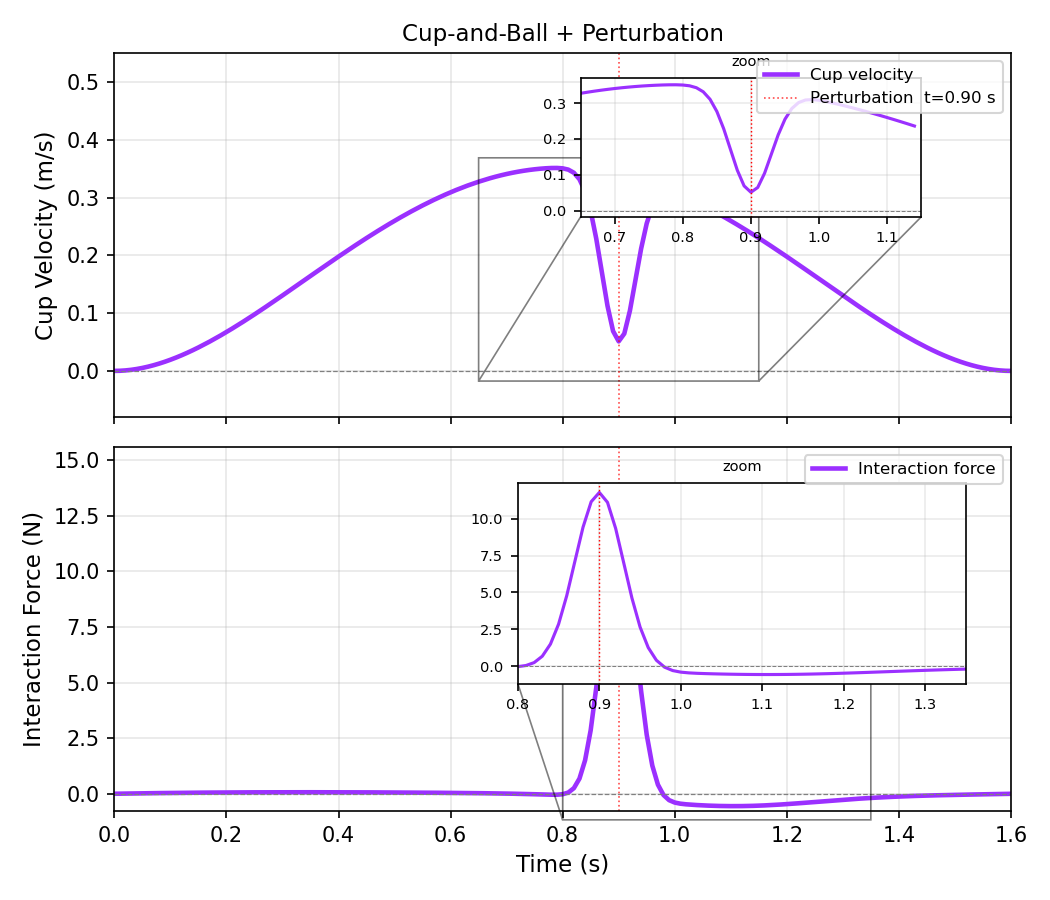
\includegraphics[width=\textwidth]{../demo_output/arm_cup_perturbation/cup_task_velocity_force_perturb.png}
  \caption{Prescribed cup velocity (top) and three-component interaction
    force $F_\text{int}(t)$ (bottom).
    The Gaussian velocity dip at $t=0.90\,\text{s}$ and the force spike
    match the purple-line reference profile.}
\end{subfigure}\hfill
\begin{subfigure}[t]{0.48\textwidth}
  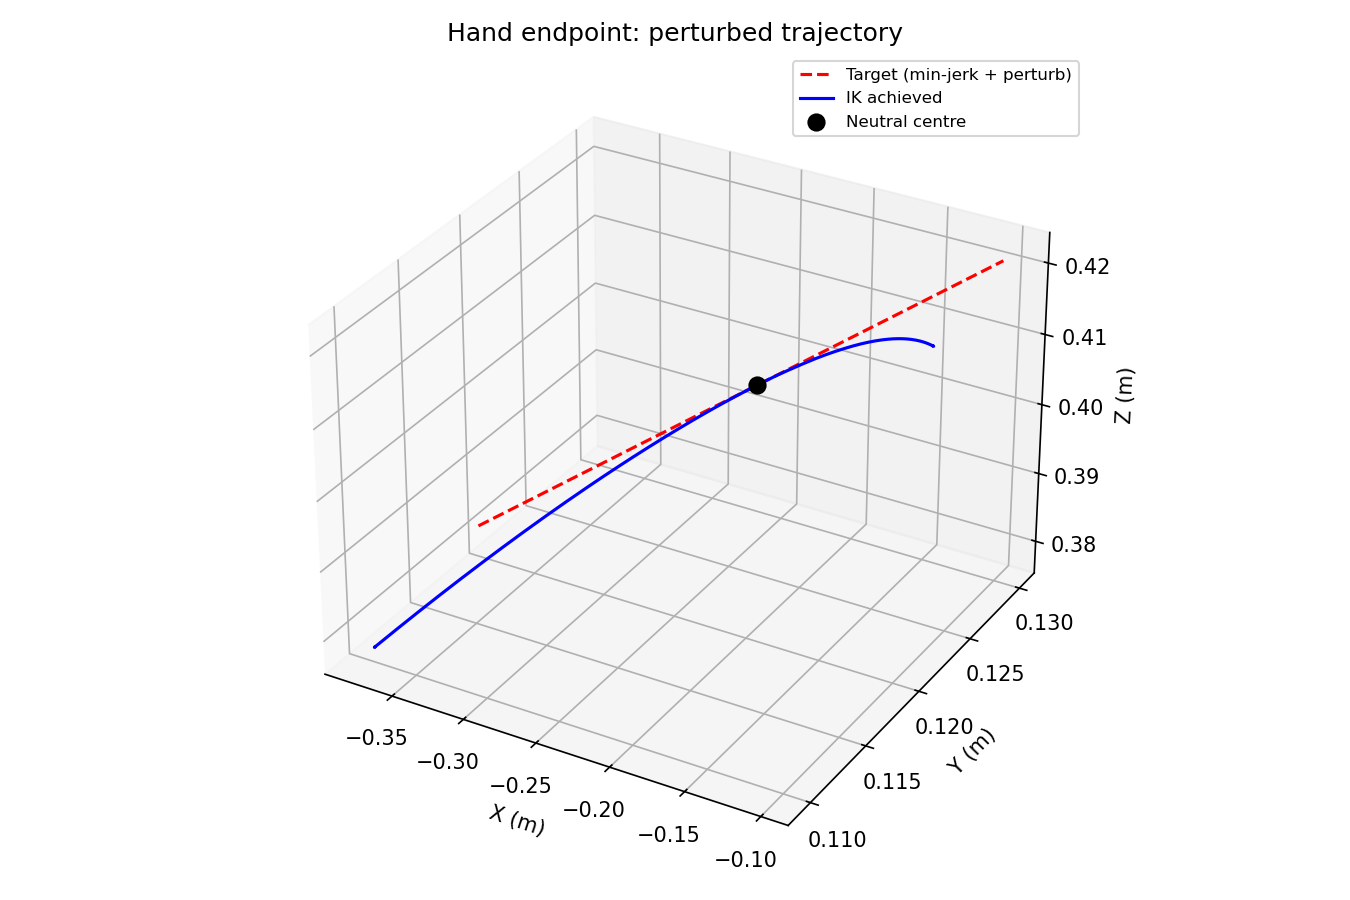
\includegraphics[width=\textwidth]{../demo_output/arm_cup_perturbation/cup_task_endpoint_path_perturb.png}
  \caption{3-D hand endpoint path (blue) vs.\ the straight horizontal
    target line (red dashed).  The small deflection from the ideal line
    reflects IK residual (${<}2\,\text{mm}$ mean).}
\end{subfigure}
\caption{Trajectory characterisation outputs from \file{arm\_cup\_perturbation.py}.}
\end{figure}

\begin{figure}[H]
\centering
\begin{subfigure}[t]{0.48\textwidth}
  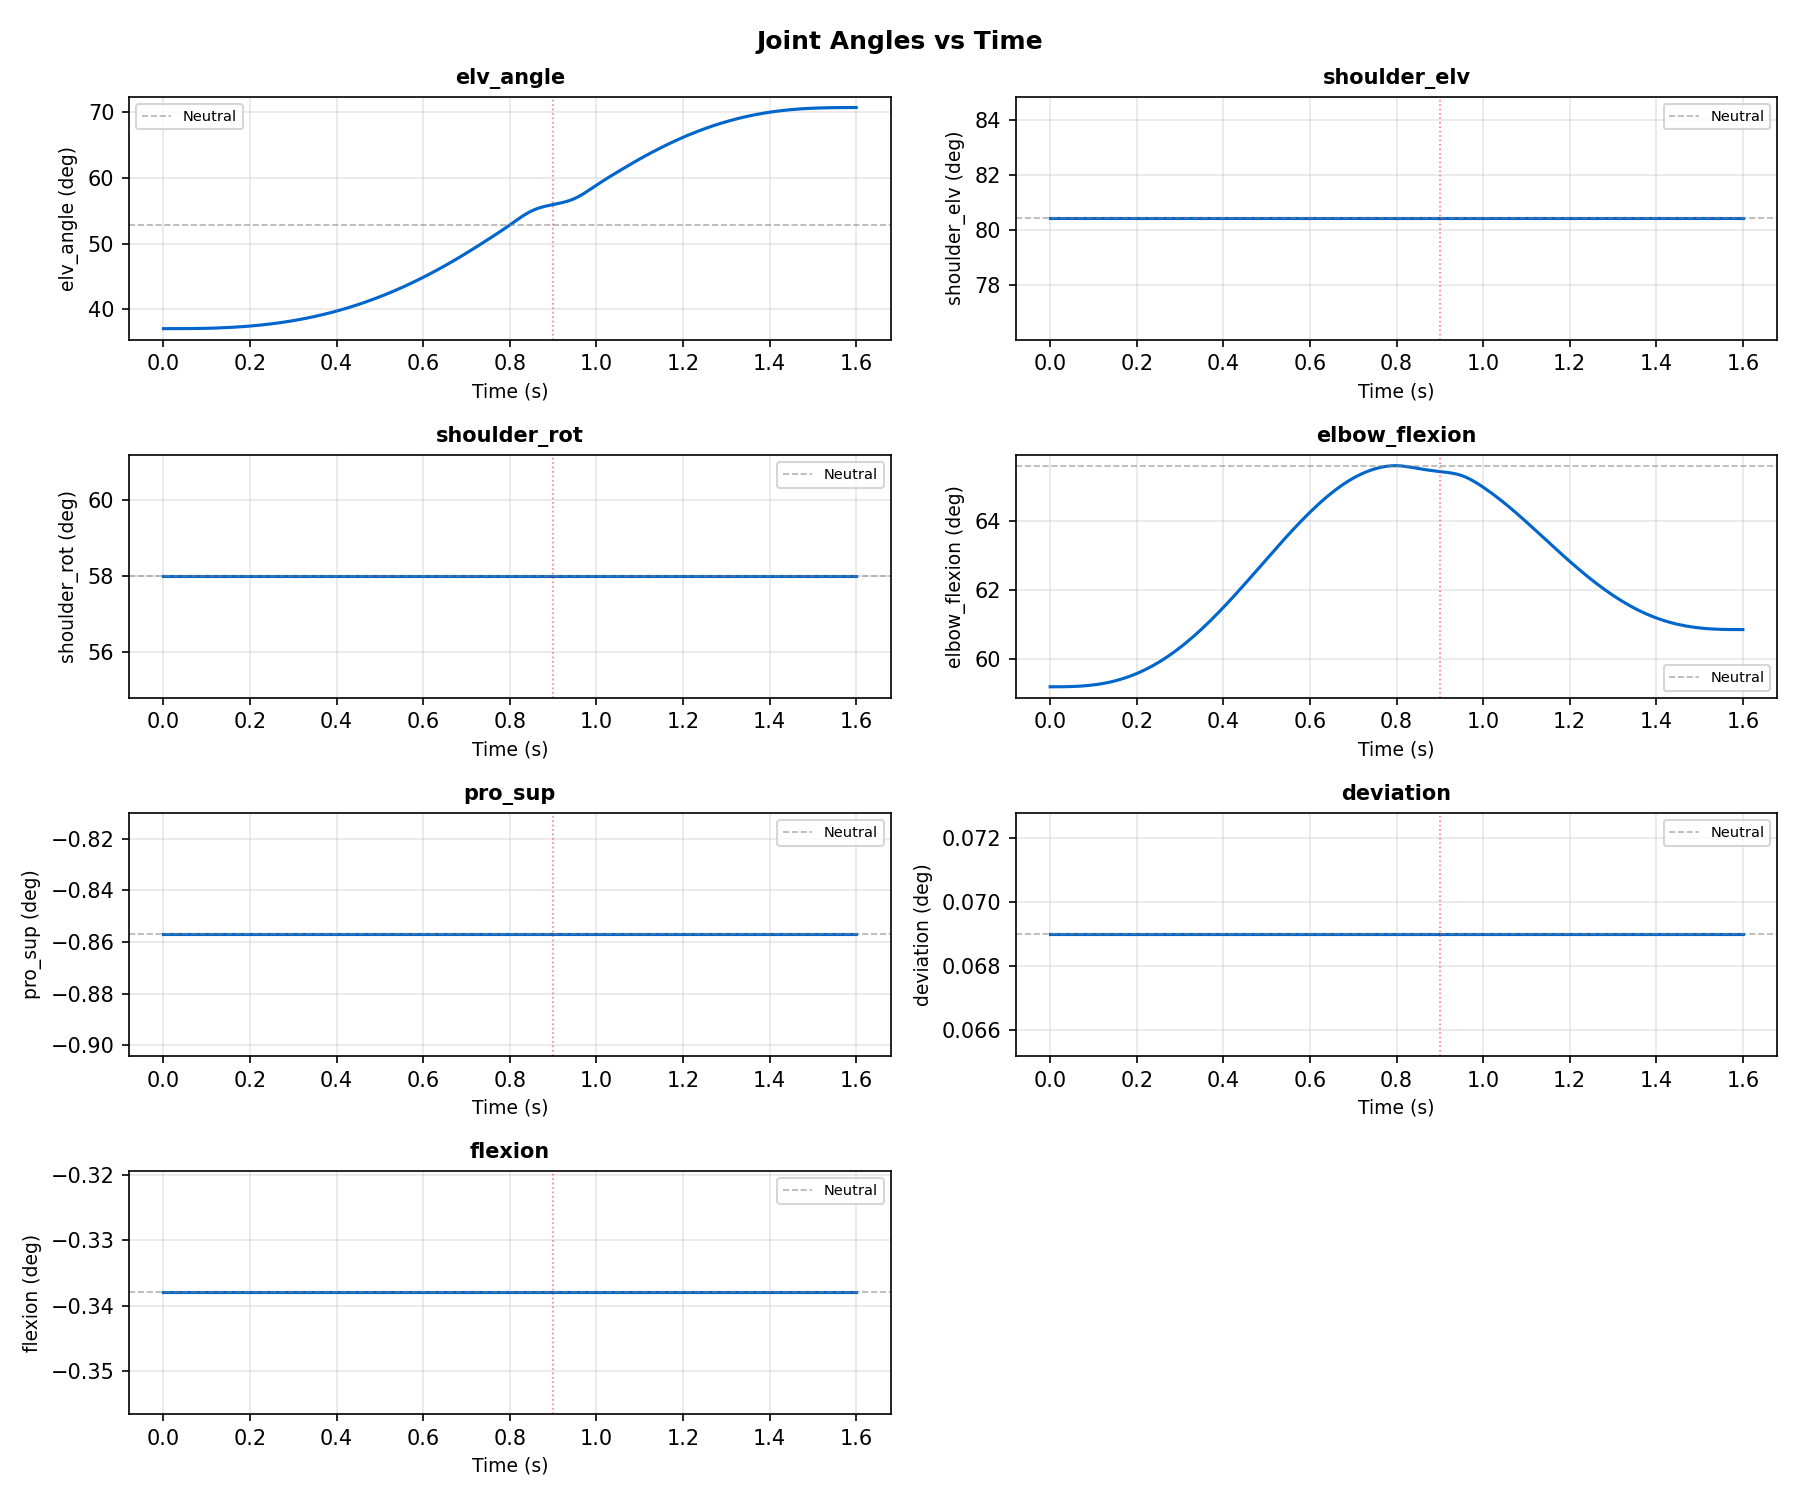
\includegraphics[width=\textwidth]{../demo_output/arm_cup_perturbation/cup_task_joint_angles_perturb.png}
  \caption{All 7 joint angles over time.  \dof{elv\_angle} and
    \dof{elbow\_flexion} are IK-solved; the others are locked at neutral.}
\end{subfigure}\hfill
\begin{subfigure}[t]{0.48\textwidth}
  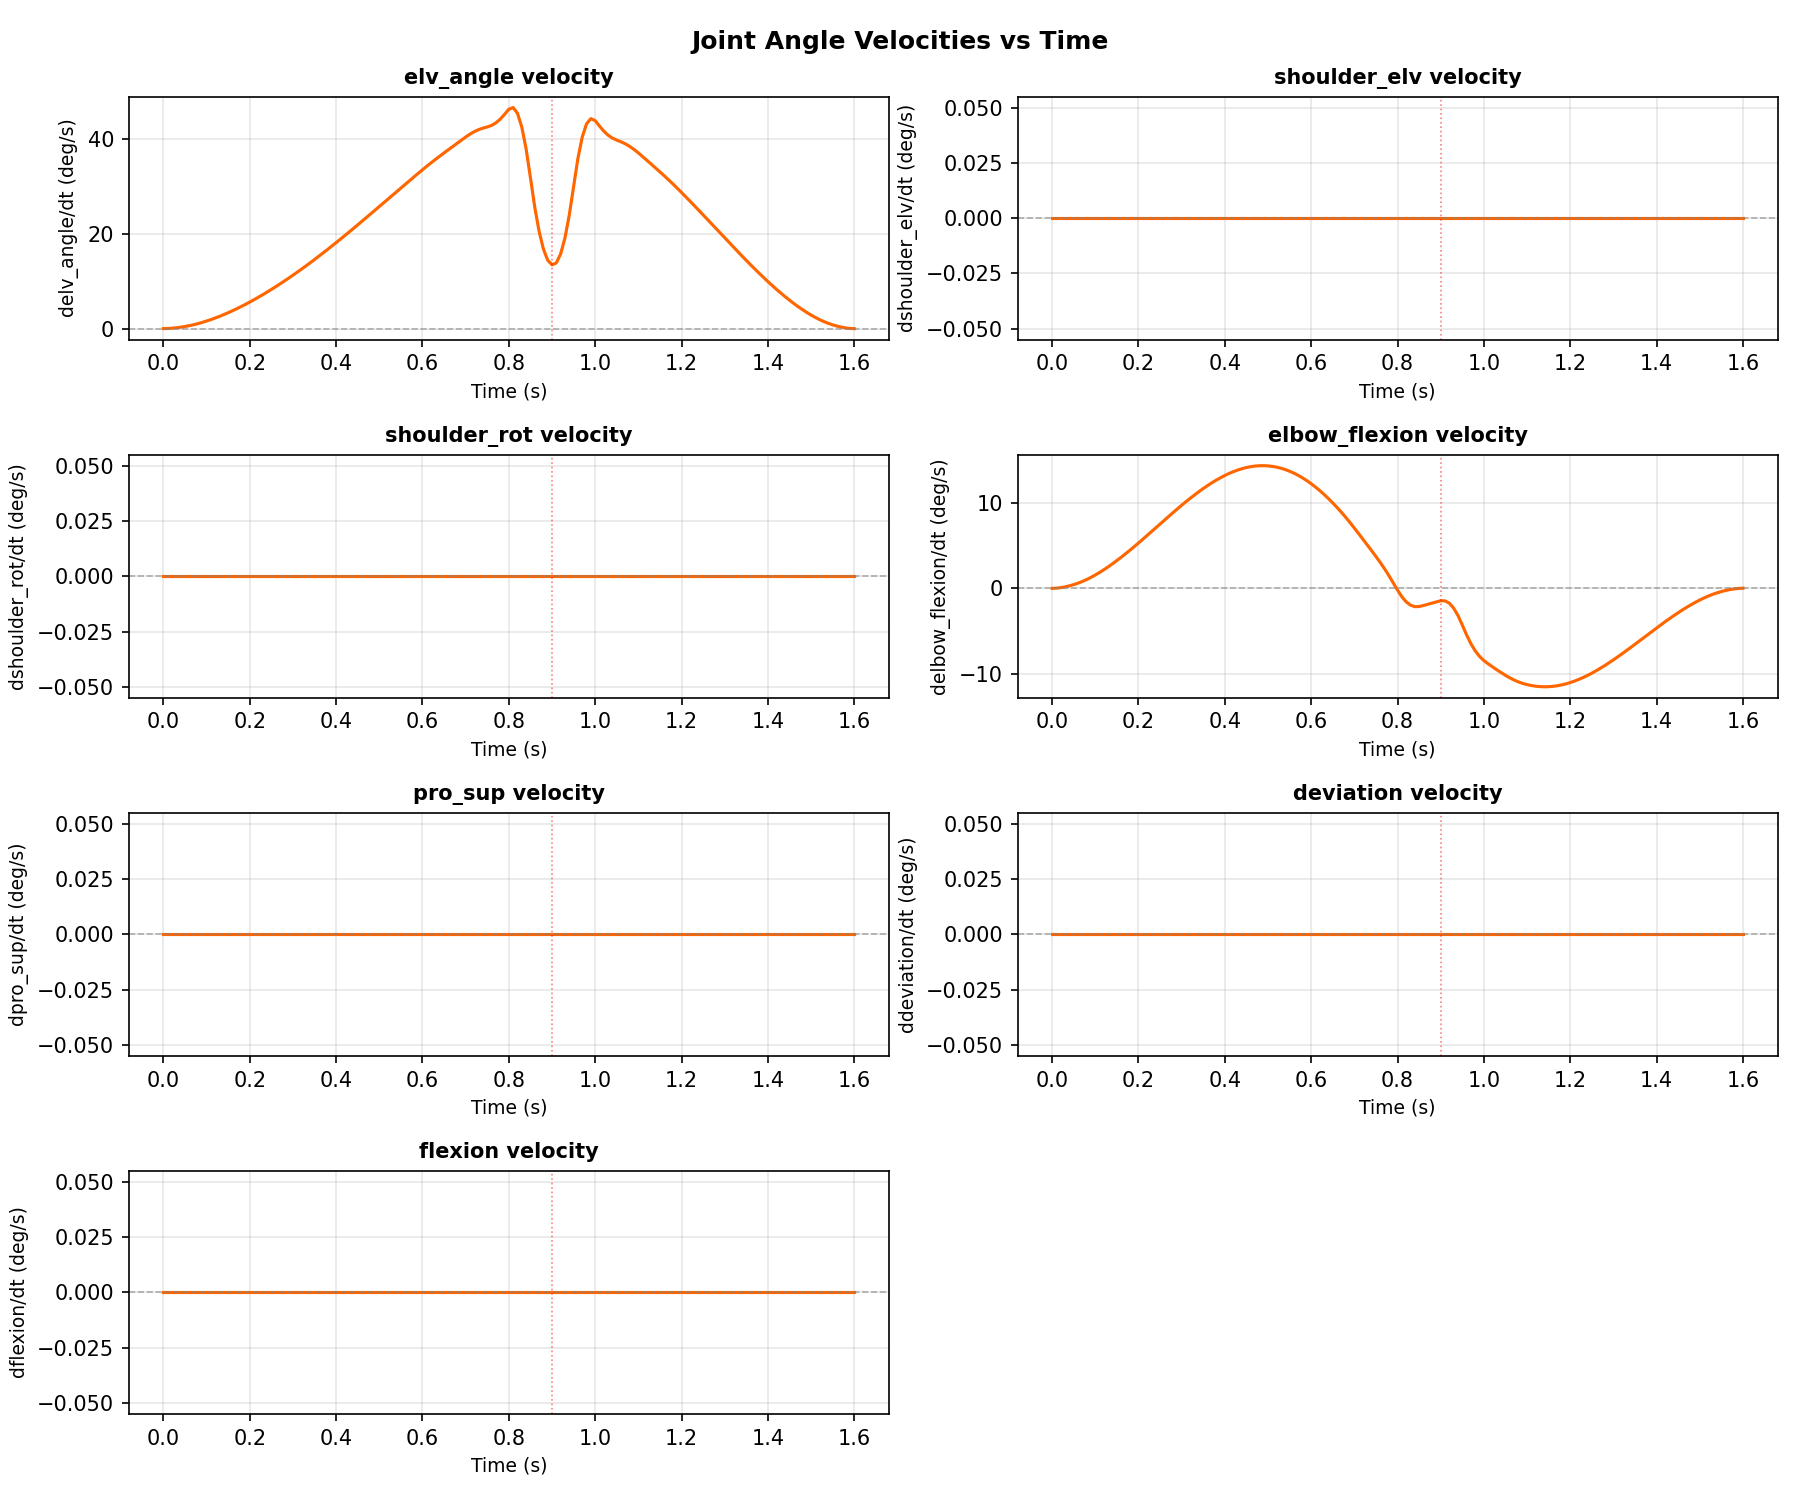
\includegraphics[width=\textwidth]{../demo_output/arm_cup_perturbation/cup_task_joint_velocities_perturb.png}
  \caption{Joint angle velocities.  The sharp velocity transient at
    $t_\text{pert}$ is visible in both IK-solved DOFs.}
\end{subfigure}
\caption{IK-solved kinematic outputs.}
\end{figure}

\begin{figure}[H]
\centering
\begin{subfigure}[t]{0.48\textwidth}
  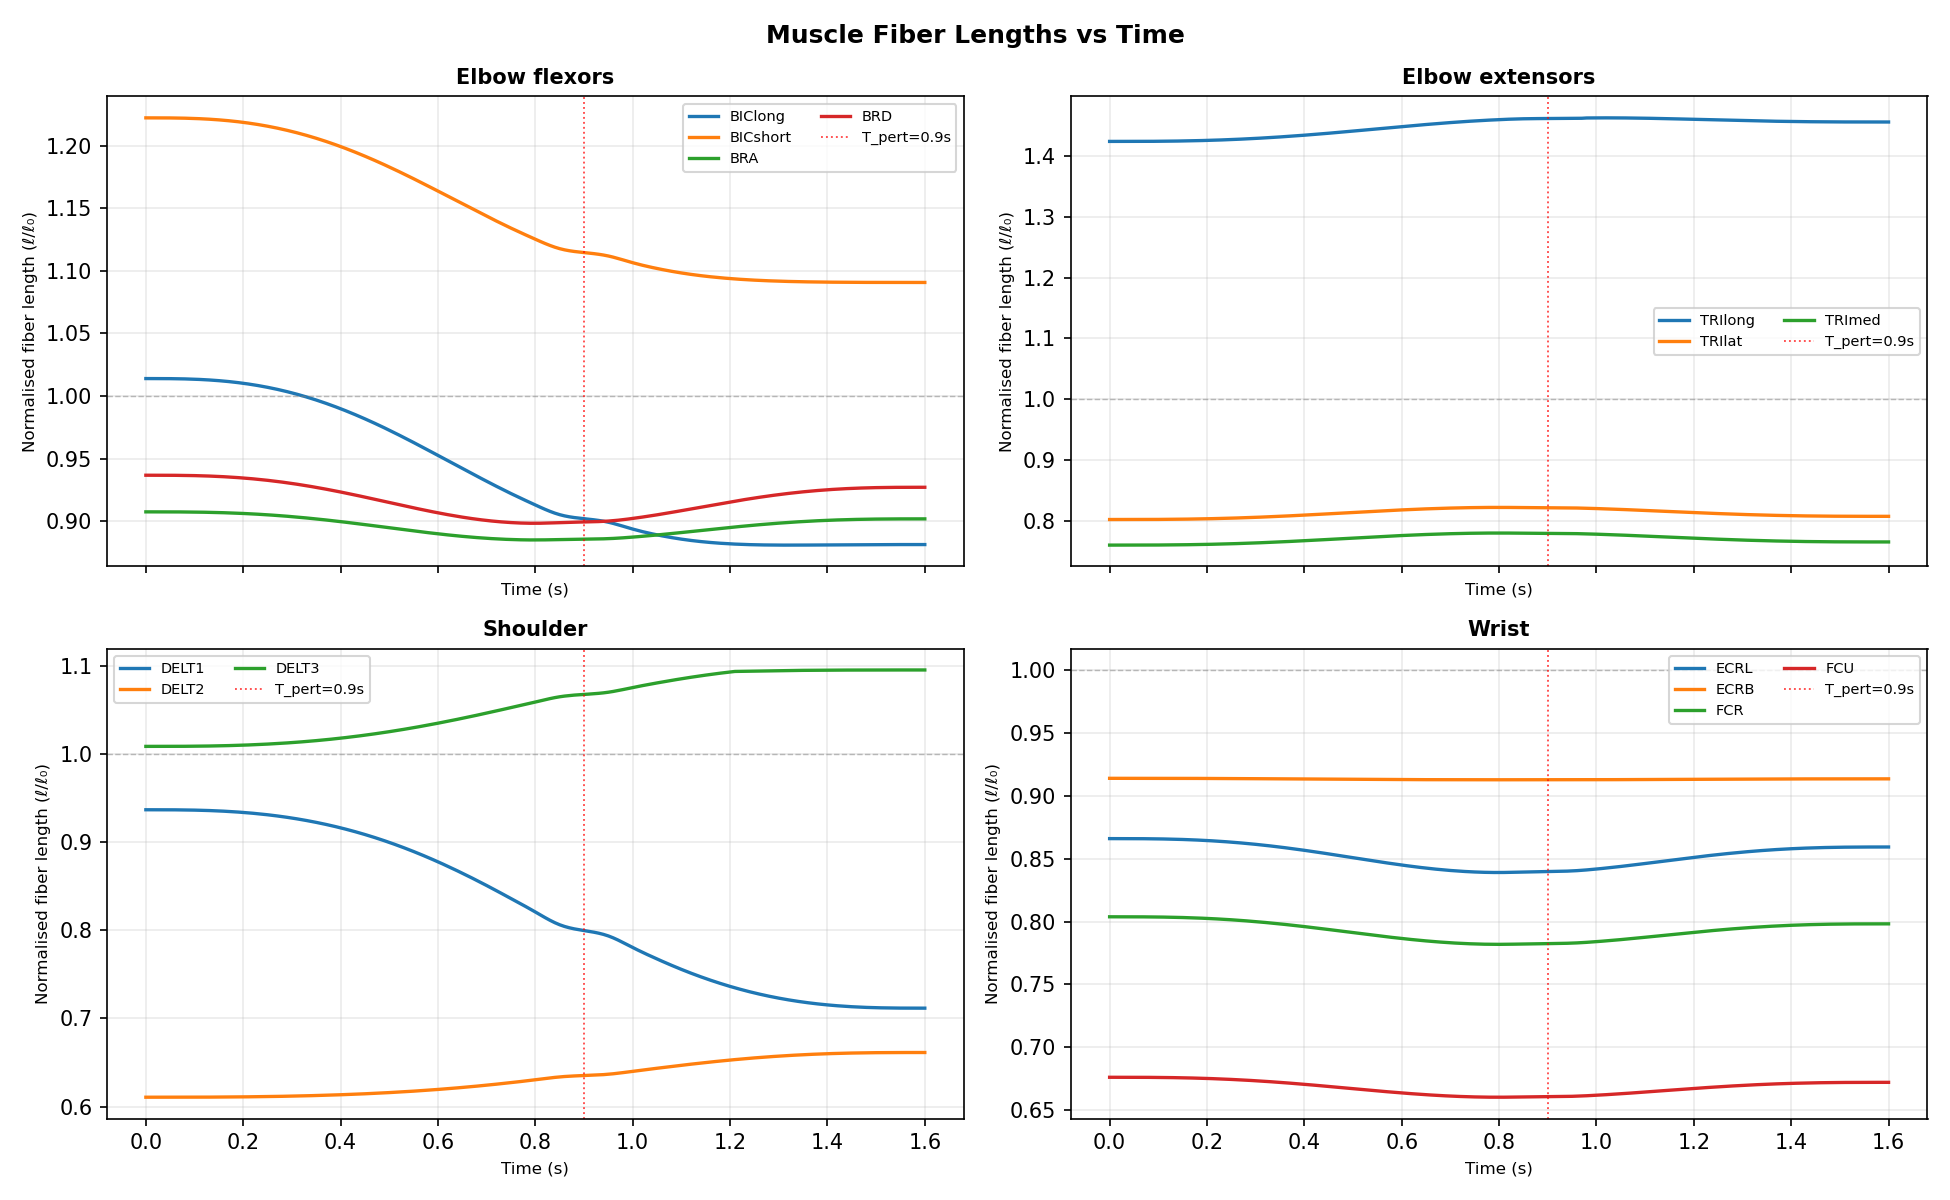
\includegraphics[width=\textwidth]{../demo_output/arm_cup_perturbation/cup_task_fiber_lengths_perturb.png}
  \caption{Normalised passive fiber lengths $l_m / l_\text{opt}$ for all
    14 tracked muscles.  Values near 1.0 indicate the muscle operates
    close to its optimal length (maximum force capacity).}
\end{subfigure}\hfill
\begin{subfigure}[t]{0.48\textwidth}
  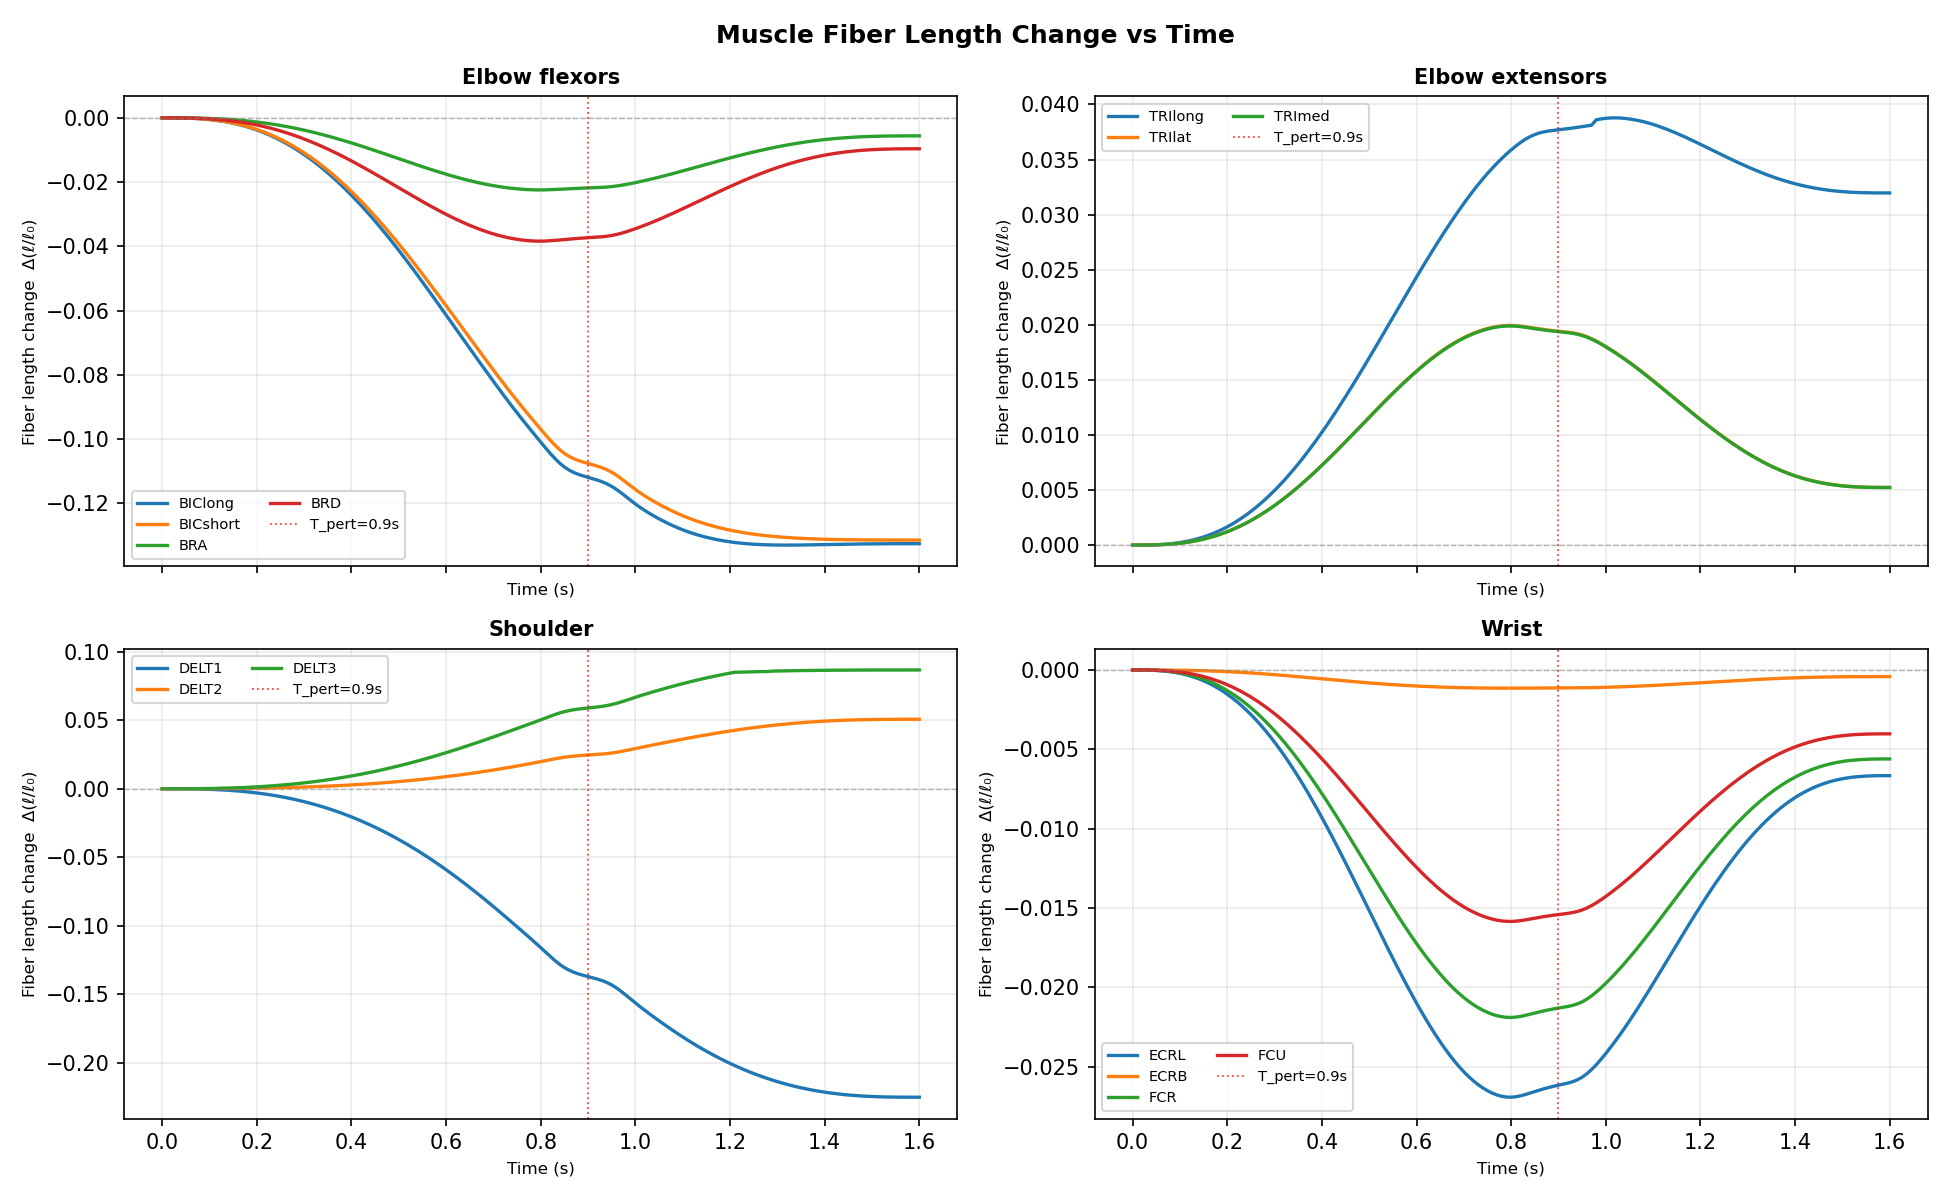
\includegraphics[width=\textwidth]{../demo_output/arm_cup_perturbation/cup_task_fiber_length_change_perturb.png}
  \caption{Fiber length \emph{change} relative to the first frame, showing
    which muscles are lengthened/shortened during the movement.}
\end{subfigure}
\caption{Passive fiber length outputs (no muscle activation assumed).}
\end{figure}


% ============================================================
\section{\texttt{arm\_inverse\_dynamics.py} — ID + Static Optimisation}
% ============================================================

\file{arm\_inverse\_dynamics.py} (class \py{ArmInverseDynamics}) reads the
IK trajectory from \file{arm\_cup\_perturbation.py}, applies the measured
interaction force as an external wrench on the hand body, runs OpenSim
\texttt{InverseDynamicsTool} to obtain joint torques, then uses Static
Optimisation to decompose those torques into individual muscle activations.
All numerical constants (\py{BASELINE\_ALPHA}, \py{ACTIVE\_IK\_DOFS},
\py{HAND\_BODY}, IK bounds, perturbation timing) are imported from
\file{config.py}.

\subsection{External Wrench Formulation}

\begin{eqbox}{Force on hand body (Newton's 3rd law)}
The participant's hand pushes \emph{against} the perturbation force:
\begin{equation}
\bm{F}_\text{on hand}(t) = -F_\text{int}(t)\,\hat{\bm{d}}(t)
\end{equation}
where $\hat{\bm{d}}(t)$ is the unit direction of motion in the ground frame,
computed frame-by-frame from the Jacobian.

\medskip
\textbf{Why include the inertial baseline?}
The cup+ball inertia ($M_\text{eff}\ddot{x}_\text{mj}$) is \emph{not} part of
the arm's rigid body model, so it must enter as an external load.
The arm's own inertia is handled internally by OpenSim's Newton--Euler equations.
\end{eqbox}

\subsection{Inverse Dynamics}

\begin{eqbox}{Newton--Euler ID}
OpenSim's \texttt{InverseDynamicsTool} solves for the generalised forces
$\btau(t) \in \R^{n_\text{dof}}$ that satisfy:
\begin{equation}
\bm{M}(\bq)\ddot{\bq} + \bm{C}(\bq,\dot{\bq}) + \bm{G}(\bq)
= \btau + \bm{J}^T\bm{F}_\text{ext}
\end{equation}
given $\bq(t)$, $\dot{\bq}(t)$, $\ddot{\bq}(t)$ from the motion file
(spline-differentiated, low-pass at 6\,Hz).
\end{eqbox}

\subsection{Force Recovery Check}

\begin{eqbox}{Interaction force recovery (loop-closure)}
Running a \emph{baseline} ID with no external force gives $\btau_0(t)$.
The difference $\Delta\btau = \btau - \btau_0$ contains only the external-force
contribution.  Projecting onto the Jacobian direction:
\begin{equation}
\bm{j}_\text{line} = \bm{J}^T\hat{\bm{d}} \in \R^2
\qquad
F_\text{int}^\text{rec}(t)
  = \frac{\bm{j}_\text{line}^\top \Delta\btau}
         {\bm{j}_\text{line}^\top \bm{j}_\text{line}}
\end{equation}
A match between $F_\text{int}^\text{rec}$ and the prescribed $F_\text{int}$
validates the wrench formulation.
\end{eqbox}

\subsection{\texttt{compute\_jacobian} — Central-Difference Jacobian}

The numerical Jacobian is used both for the external-wrench loop-closure check
and as input to the stiffness mapping in \file{compute\_stiffness.py}.

\begin{eqbox}{\texttt{compute\_jacobian(model, state, q)} $\to$ $\bm{J}\in\R^{3\times2}$}
For each of the two IK-active DOFs ($j \in \{\text{elv\_angle},\,\text{elbow\_flexion}\}$):
\begin{equation}
J_{ij}(t) = \frac{\partial p_i}{\partial q_j}
  \;\approx\; \frac{\mathrm{FK}_i(q + \varepsilon\,\bm{e}_j)
                  - \mathrm{FK}_i(q - \varepsilon\,\bm{e}_j)}{2\varepsilon},
\quad \varepsilon = 10^{-6}\,\text{rad}
\end{equation}
where $i \in \{x,y,z\}$ is the Cartesian hand coordinate and
$\mathrm{FK}$ evaluates the ground-frame hand position
via \texttt{findStationLocationInGround}.
The Jacobian is \emph{rectangular} ($3\times2$) because only 2 DOFs are IK-solved
in \file{arm\_inverse\_dynamics.py}.
\end{eqbox}

\subsection{Static Optimisation — \texttt{run\_active\_msk()}}

Static Optimisation (SO) decomposes the joint torques into individual muscle
activations under the minimum-effort criterion.  The per-frame computation
inside \texttt{run\_active\_msk()} is:

\begin{eqbox}{Per-frame SO loop body — \texttt{run\_active\_msk()}}
\textbf{Step 1}: Set all 7 DOFs from trajectory row $\bq_i$; realise to Velocity.

\textbf{Step 2}: Query OpenSim's Hill active force--length multiplier:
\begin{equation}
fl_m = \texttt{getActiveForceLengthMultiplier}(\text{state})
\qquad\in [0,1]
\end{equation}
(OpenSim Hill model — tabulated, not Gaussian; depends on full Hill equilibrium.)

\textbf{Step 3}: Moment arm matrix ($n_\text{dof}=2$ here):
\begin{equation}
R_{im} = \texttt{computeMomentArm}(\text{state},\,\text{coord}_i)
\quad\Rightarrow\quad
\bR \in \R^{2\times14}
\end{equation}

\textbf{Step 4}: Static Optimisation (shared \texttt{so\_frame}):
\begin{equation}
\ba^*(t) = \arg\min_{\ba}\;\|\ba\|_2^2 \qquad
\text{s.t.}\quad \bR\,(\ba\odot\bF_0\odot\bm{fl}) = \btau_i,
\quad 0 \leq a_m \leq 1
\end{equation}

\textbf{Step 5}: Set activations, \texttt{equilibrateMuscles}, read $l_m(t)$:
\begin{equation}
\tilde{l}_m(t) = \frac{\texttt{getFiberLength}(\text{state})}{l_{\text{opt},m}}
\end{equation}

\textbf{Step 6}: Hill stiffness linearisation ($\beta = 40$, dimensionless):
\begin{equation}
k_m^{\text{Hill}} = \beta \cdot a_m \cdot F_{0,m} \cdot fl_m \;/\; l_{\text{opt},m}
\qquad\bigl[\text{N/m}\bigr]
\end{equation}

\textbf{Step 7}: Joint stiffness assembly:
\begin{equation}
\bK_\text{joint}(t) = \bR(t)\,\mathrm{diag}\!\left(k_m^{\text{Hill}}\right)\bR(t)^\top
  \;\in\; \R^{2\times2}
\end{equation}

\textbf{Step 8}: Co-contraction index (elbow muscle groups):
\begin{equation}
A_\text{flex}(t) = \sum_{m\in\{\text{BIC, BRA, BRD}\}} a_m(t),
\qquad
A_\text{ext}(t)  = \sum_{m\in\{\text{TRI}\}} a_m(t)
\end{equation}
\begin{equation}
\text{CCI}(t) = \frac{2\min\bigl(A_\text{flex},\,A_\text{ext}\bigr)}
                     {A_\text{flex} + A_\text{ext} + \varepsilon},
\quad \varepsilon = 10^{-9}
\end{equation}
\end{eqbox}

\begin{notebox}[PipeBlue]{Numerical example --- SO loop at $t=0.90\,\text{s}$ (perturbation peak)}
Representative per-muscle values from the SO solution at this frame:
\begin{center}\small
\begin{tabular}{llllll}
\toprule
Muscle & $a_m$ & $F_{0,m}$ & $fl_m$ & $L_{\text{opt},m}$ & $k_m^{\text{Hill}}$ (\textbf{with} $\beta=40$) \\
\midrule
\rowcolor{LightBlue}
BIClong & 0.50 & 629\,N & 0.90 & 0.116\,m &
  $40\times0.50\times629\times0.90/0.116\approx\mathbf{97{,}500}\,\text{N/m}$ \\
TRIlong & 0.05 & 798\,N & 0.70 & 0.127\,m &
  $40\times0.05\times798\times0.70/0.127\approx\mathbf{8{,}800}\,\text{N/m}$ \\
\bottomrule
\end{tabular}
\end{center}
Elbow-axis diagonal contributions
($R_\text{BIC,ef}\approx0.045\,\text{m}$, $R_\text{TRI,ef}\approx0.025\,\text{m}$):
\[
K_\text{joint,ef,ef}^{\text{BIC}} = (0.045)^2\times97{,}500 \approx 197\,\text{N}{\cdot}\text{m/rad}
\qquad
K_\text{joint,ef,ef}^{\text{TRI}} = (0.025)^2\times8{,}800 \approx 5.5\,\text{N}{\cdot}\text{m/rad}
\]
Summing all 14 muscles gives a typical $K_\text{joint,ef,ef}\approx200\text{--}500\,\text{N}{\cdot}\text{m/rad}$
during the perturbation window (elevated by the stiffness spike).\\[4pt]
\textbf{CCI at this frame}:
$A_\text{flex}=0.50+0.10+0.12=0.72$, $A_\text{ext}=0.05+0.03+0.04=0.12$
\[
\text{CCI} = \frac{2\times0.12}{0.72+0.12} = \frac{0.24}{0.84} = \mathbf{0.29}
\]
A CCI of $0.29$ indicates moderate co-contraction: extensors are only $29\%$
as active as they would need to be for fully balanced co-contraction ($\text{CCI}=1$).
\end{notebox}

\begin{notebox}[PipeOrange]{Comparison vs.\ \file{compute\_stiffness.py}}
Both scripts now produce the endpoint stiffness $\bm{K}_e(t) \in \R^{3\times3}$
and its principal eigenvalues $\lambda_\text{min},\,\lambda_\text{max}$
(major/minor axes of the XY stiffness ellipse, the quantities that
Tele-Impedance Stage~2 calibrates from EMG, Ajoudani et al.\ 2012).
The two scripts differ in three ways:
\begin{itemize}\itemsep2pt
  \item \textbf{F\textsubscript{int}}: \file{arm\_inverse\_dynamics.py} applies
    $F_\text{int}(t)$ as an external wrench on the hand, so $\tau(t)$
    contains the cup--ball reaction (peak $\sim$30~N$\cdot$m at
    $t_\text{pert}$). \file{compute\_stiffness.py} runs ID kinematic-only.
  \item \textbf{DOFs in SO}: ID script uses 2 DOFs
    (\dof{elv\_angle}, \dof{elbow\_flexion}); the endpoint-stiffness script
    uses all 7 active DOFs.
  \item \textbf{Hill stiffness coefficient}: ID script uses $\beta=40$;
    \file{compute\_stiffness.py}'s \texttt{\_endpoint\_stiffness()} uses
    $\beta=1$. Joint-stiffness magnitudes therefore differ by $\sim40\times$,
    but both produce the same qualitative $\bm{K}_e$ modulation.
\end{itemize}
\end{notebox}

\begin{notebox}[PipePurple]{Output files — \outdir{demo\_output/arm\_inverse\_dynamics/}}
\begin{tabular}{ll}
\py{cup\_task\_id\_results\_perturb.csv}          & $\tau(t), \tau_0(t), F^\text{rec}_\text{int}(t)$ \\
\py{cup\_task\_active\_fiber\_lengths\_perturb.csv} & Norm. fiber lengths $l_m/l_\text{opt}$ (with activation) \\
\py{cup\_task\_activations\_perturb.csv}           & $a_m(t)$ for all 14 muscles \\
\py{cup\_task\_joint\_stiffness\_perturb.csv}      & $K_\text{elv}, K_\text{ef}, K_\text{cross}, \bm{K}_e, \lambda_\text{min}, \lambda_\text{max}(t)$ \\
\end{tabular}
\end{notebox}

\subsection{Output Plots}

\begin{figure}[H]
\centering
\begin{subfigure}[t]{0.48\textwidth}
  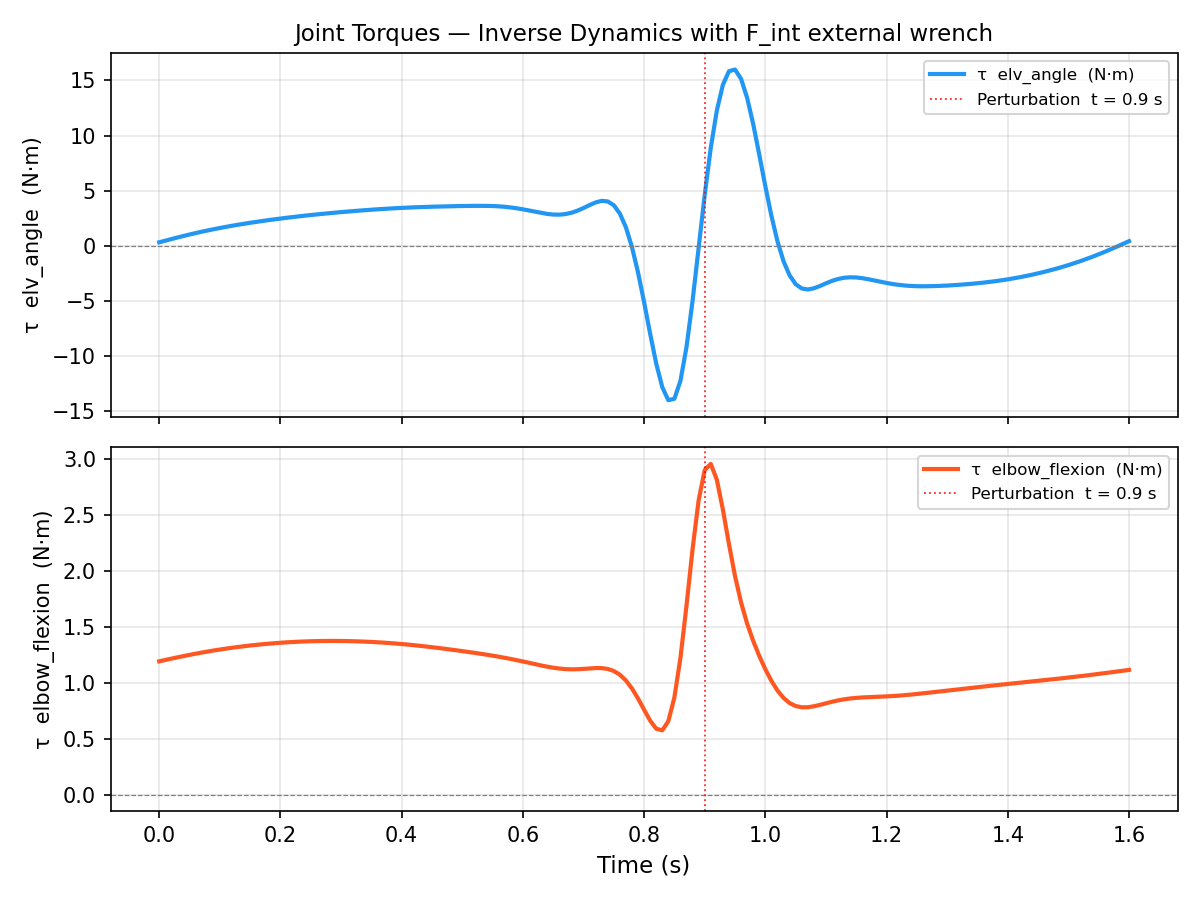
\includegraphics[width=\textwidth]{../demo_output/arm_inverse_dynamics/cup_task_id_torques_perturb.png}
  \caption{ID joint torques $\tau(t)$ for \dof{elv\_angle} and
    \dof{elbow\_flexion}.  The spike at $t_\text{pert}=0.90\,\text{s}$
    represents the demand placed on the muscles to resist the perturbation.}
\end{subfigure}\hfill
\begin{subfigure}[t]{0.48\textwidth}
  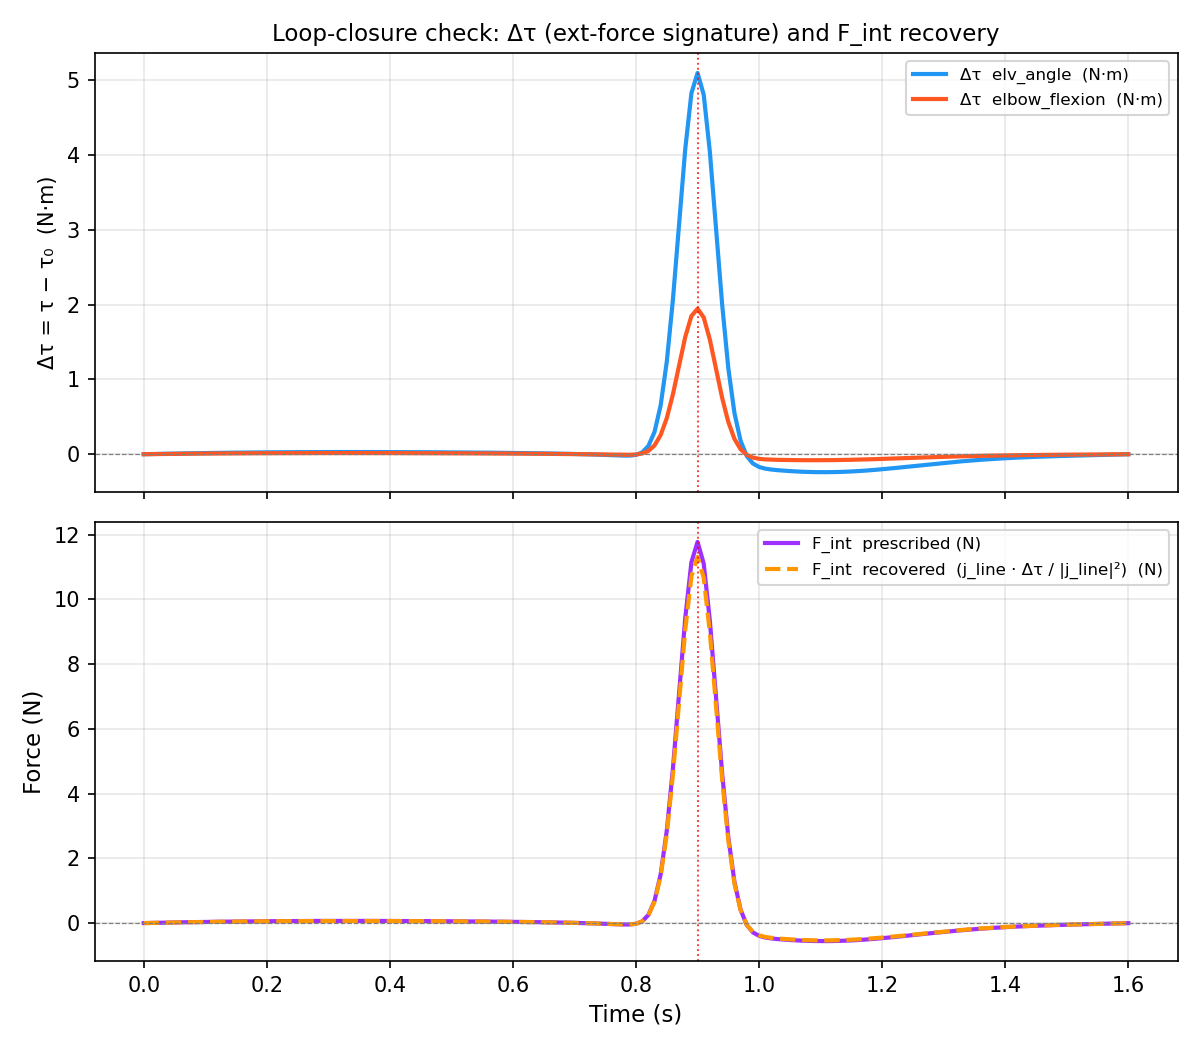
\includegraphics[width=\textwidth]{../demo_output/arm_inverse_dynamics/cup_task_id_loopclosure_perturb.png}
  \caption{Loop-closure validation: prescribed $F_\text{int}$ (blue) vs.\
    recovered $F^\text{rec}_\text{int}$ (orange dashed).
    Close agreement confirms the external wrench was correctly applied.}
\end{subfigure}
\caption{Inverse Dynamics outputs from \file{arm\_inverse\_dynamics.py}.}
\end{figure}

\begin{figure}[H]
\centering
\begin{subfigure}[t]{0.48\textwidth}
  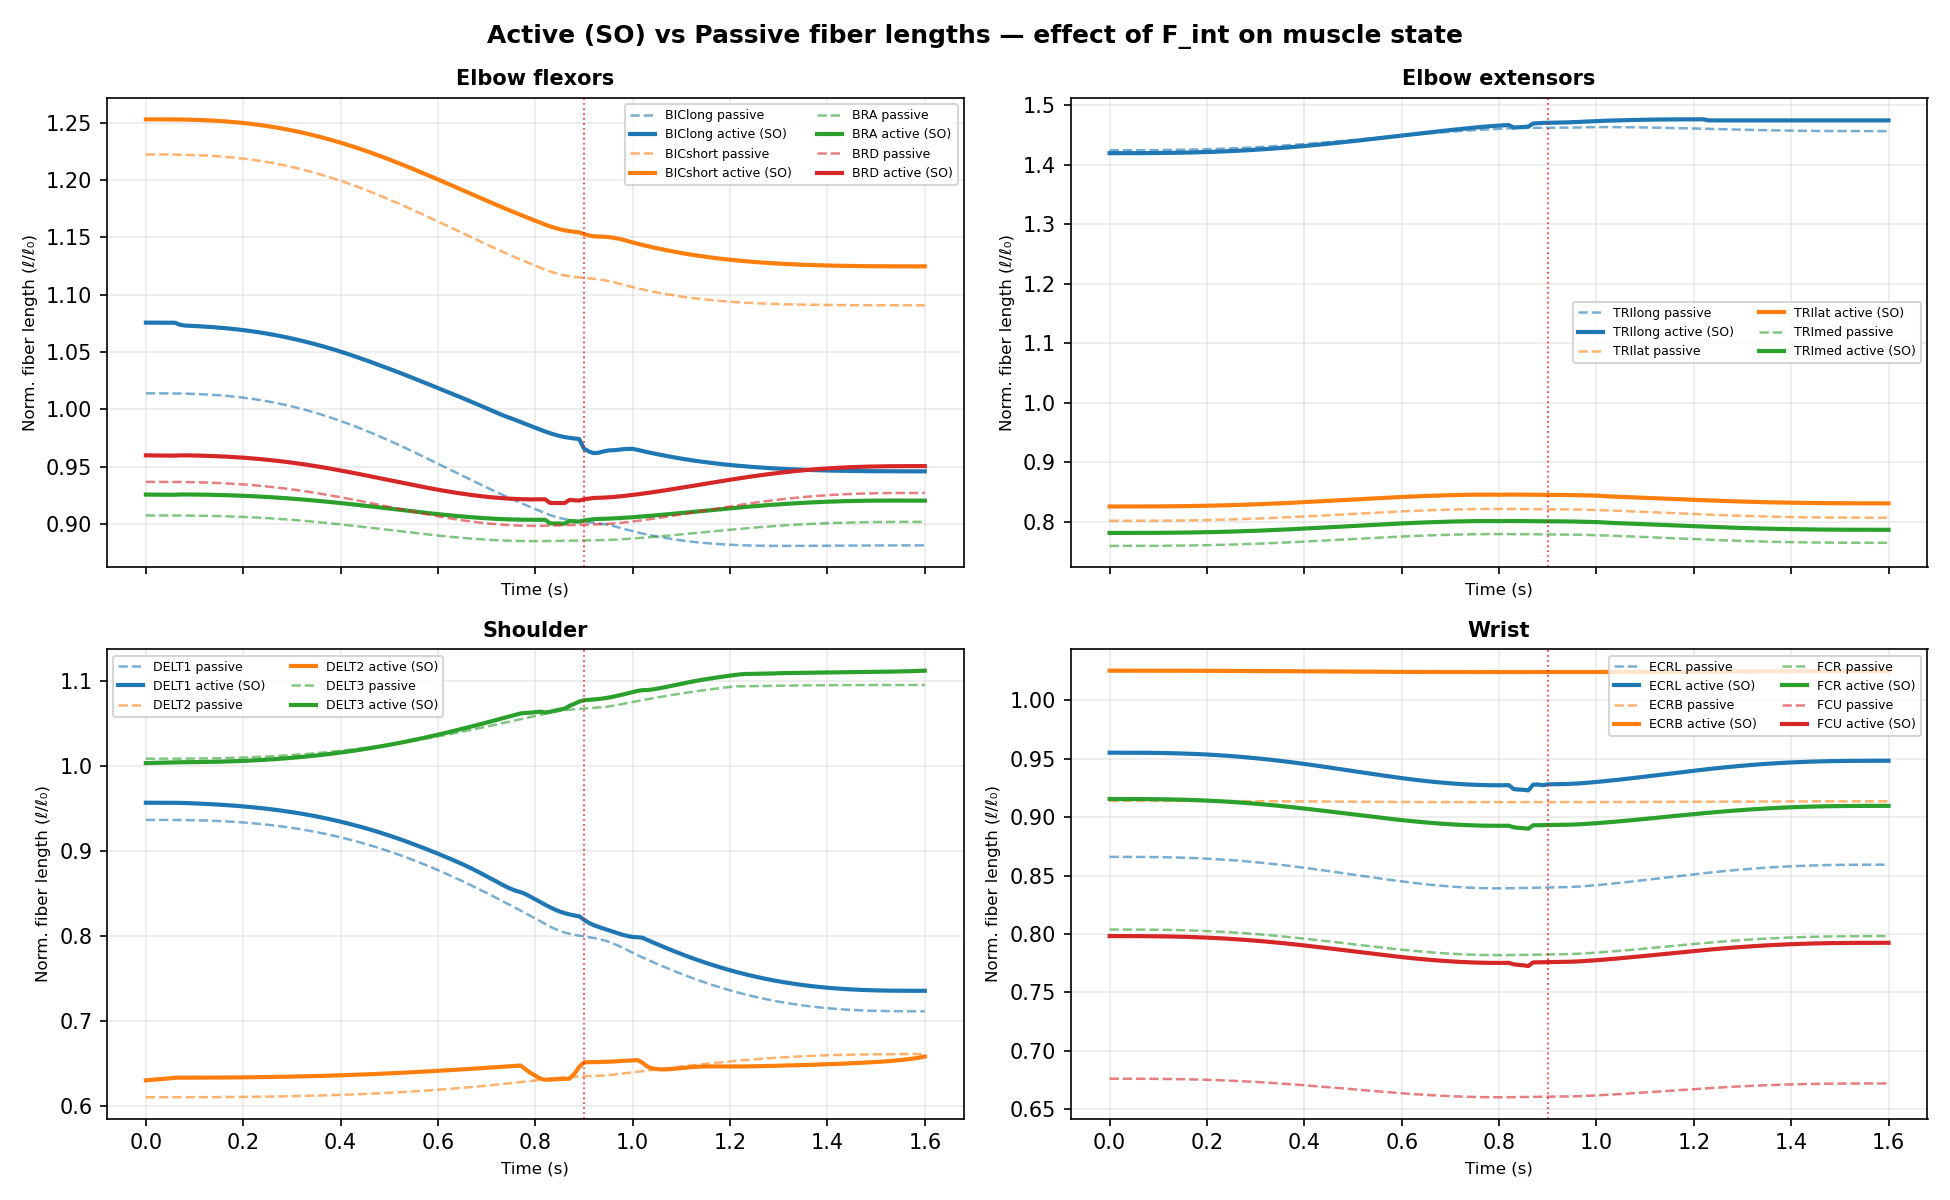
\includegraphics[width=\textwidth]{../demo_output/arm_inverse_dynamics/cup_task_active_vs_passive_fl_perturb.png}
  \caption{Active (SO, solid) vs.\ passive (no activation, dashed) normalised
    fiber lengths $l_m/l_\text{opt}$ by muscle group.
    Active lengths differ because activation shifts the fiber to a
    shorter equilibrium via the contractile element.}
\end{subfigure}\hfill
\begin{subfigure}[t]{0.48\textwidth}
  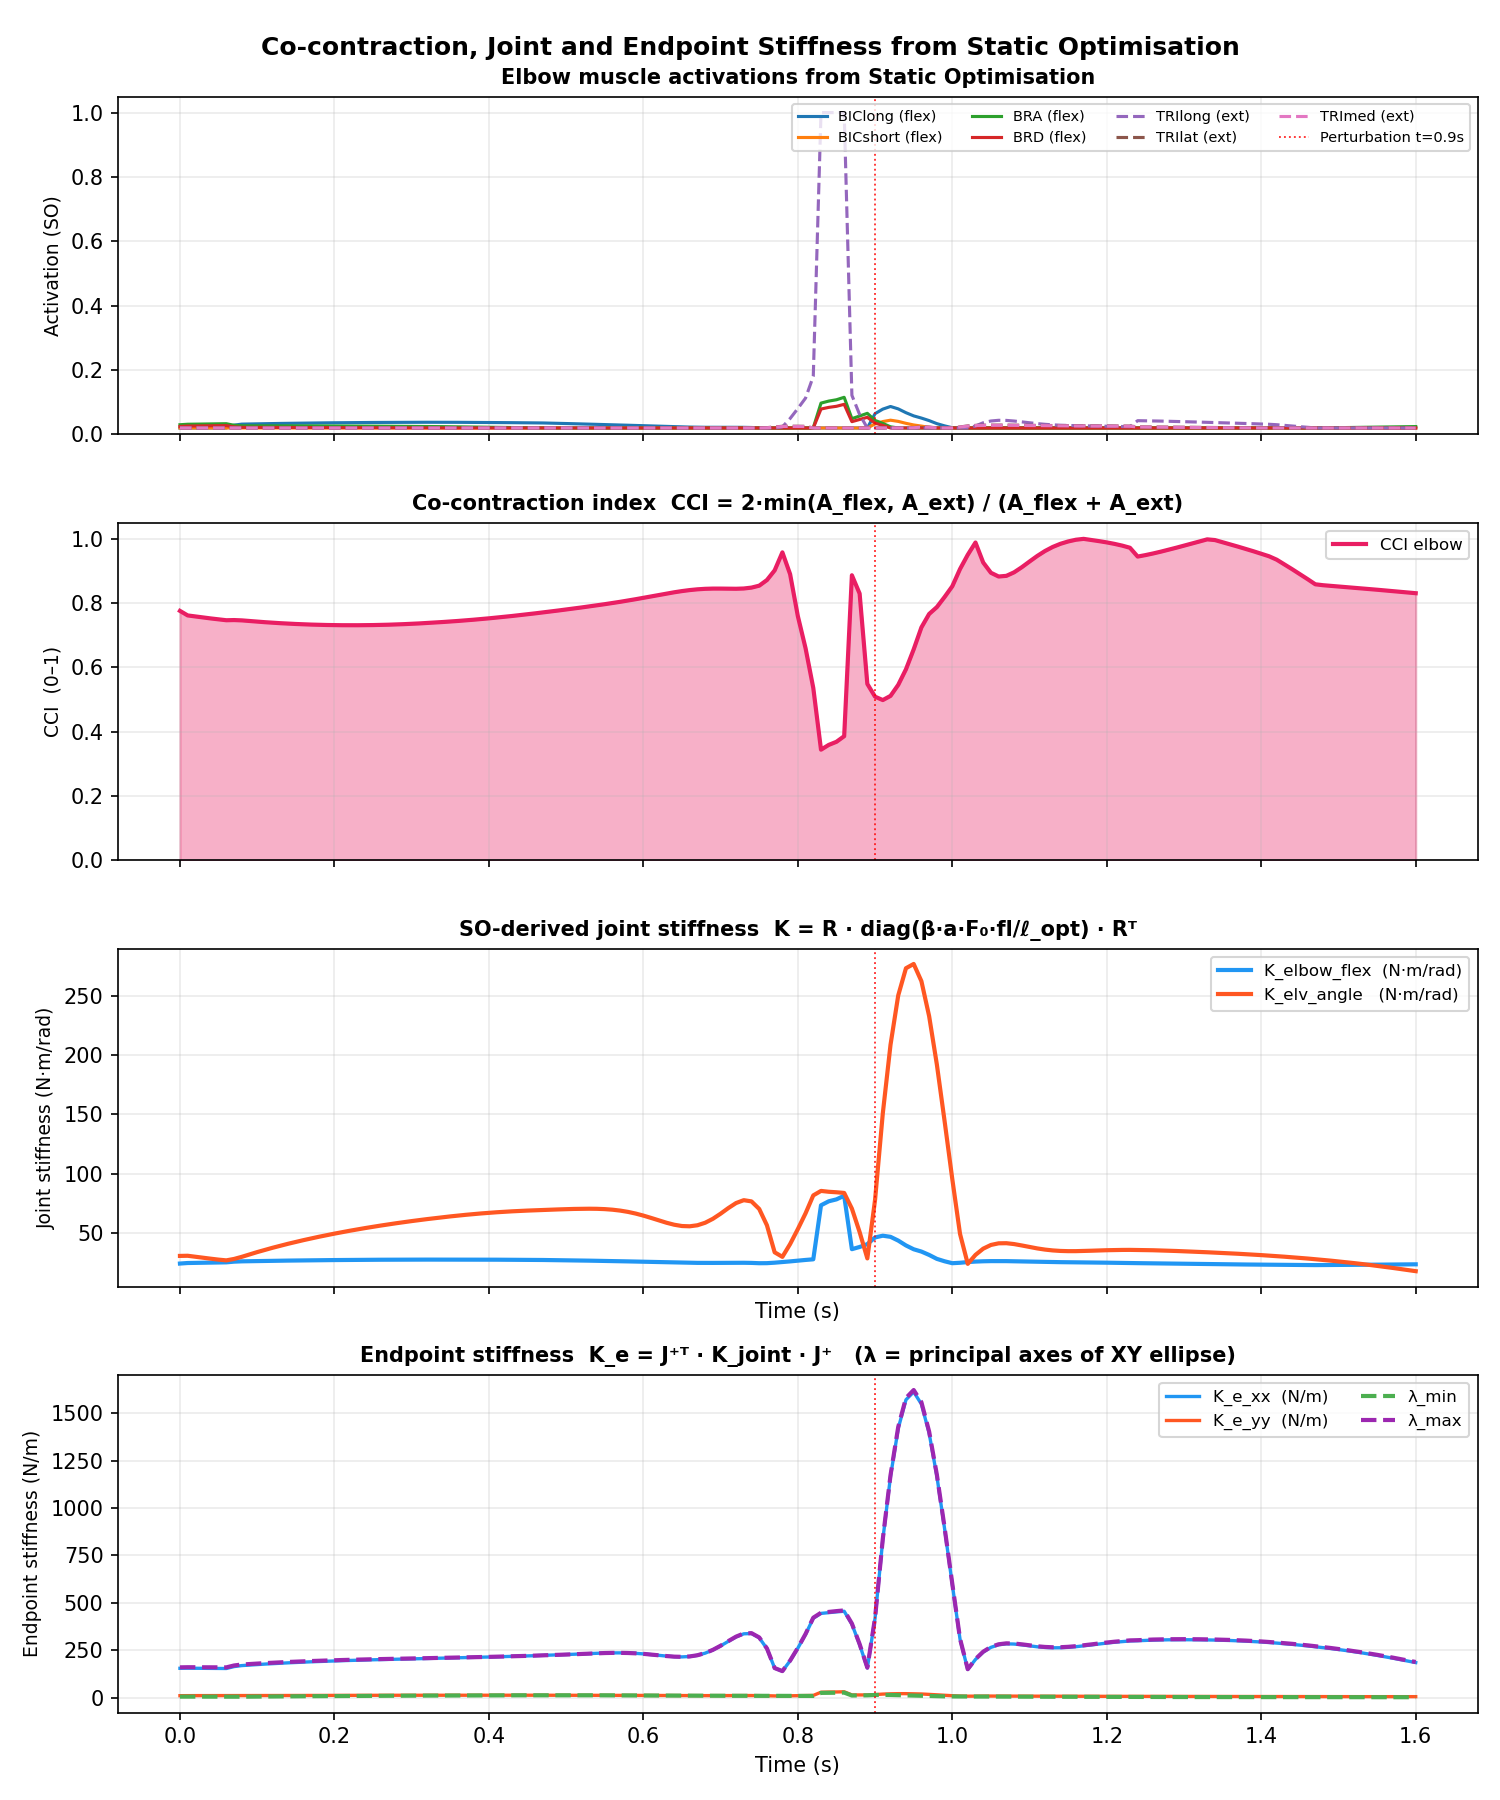
\includegraphics[width=\textwidth]{../demo_output/arm_inverse_dynamics/cup_task_cocontraction_stiffness_perturb.png}
  \caption{\textbf{Panel 1:} muscle activations (flexors solid, extensors dashed).
    \textbf{Panel 2:} CCI — rises during the perturbation window
    ($0.8$--$1.0\,\text{s}$).
    \textbf{Panel 3:} Joint stiffness $K_\text{elv\_angle}$ and $K_\text{elbow\_flex}$ [N$\cdot$m/rad];
    $K_\text{elv\_angle}$ peaks $\sim$500 driven by the $\tau_\text{elv\_angle}$ spike at $t_\text{pert}$.
    \textbf{Panel 4:} Endpoint stiffness $\bm{K}_e = J^{+\!\top}\bm{K}_\text{joint}\,J^+$ diagonals
    plus principal eigenvalues; $\lambda_\text{max}$ peaks $\sim$2900~N/m at $t_\text{pert}$
    (highly anisotropic ellipse aligned with motion direction, near-singular Jacobian at
    arm extension).}
\end{subfigure}
\caption{Static Optimisation outputs: fiber lengths, activations, co-contraction and stiffness.}
\end{figure}


% ============================================================
\section{\texttt{compute\_stiffness.py} — Endpoint Stiffness}
% ============================================================

\file{compute\_stiffness.py} (class \py{ComputeStiffness}) is the impedance
analysis hub.  It runs a complete sub-pipeline — \textbf{ID tool} $\to$
\textbf{Static Optimisation} $\to$ \textbf{Jacobian mapping} — entirely within a
single script, producing both the $3\times3$ endpoint \emph{stiffness} tensor
$\bm{K}_e(t)$ \textbf{and} the $3\times3$ endpoint \emph{damping} tensor
$\bm{D}_e(t)$ at every trajectory frame.  Two modes are available:
\texttt{static\_opt} (pure minimum-effort activations) and \texttt{cmc}
(adds a co-contraction floor during perturbation windows to model defensive
stiffening). Hill constants ($\beta_D$, $V_\text{max,factor}$, $\gamma$,
$\alpha_\text{floor}$, \py{HAND\_BODY}) are imported from \file{config.py}.

\subsection{\texttt{\_build\_ms\_properties} — Muscle Geometry per Frame}

\begin{eqbox}{\texttt{\_build\_ms\_properties(model, state, ms\_labels)}
  $\to$ $(R,\,F_\text{max},\,fl,\,L_\text{opt},\,l_m)$}
At the current OpenSim state (Position-realised), for each muscle $m$:

\textbf{1.\ Optimal fiber length} (model constant, no state):
\begin{equation}
L_{\text{opt},m} = \texttt{getOptimalFiberLength}()
\qquad [\text{m}]
\end{equation}

\textbf{2.\ Raw fiber length} (requires at least Position-realised state):
\begin{equation}
l_m = \texttt{getFiberLength}(\text{state})
\qquad [\text{m}]
\end{equation}

\textbf{3.\ Gaussian force--length multiplier} (analytic, unlike OpenSim's
tabulated Hill FL):
\begin{equation}
\boxed{fl_m = \exp\!\left(-\!\left(\frac{l_m/L_{\text{opt},m} - 1}{\gamma}\right)^{\!2}\right)},
\qquad \gamma = 0.45
\end{equation}
\begin{itemize}\itemsep0pt
  \item $l_m = L_\text{opt}$: $fl = 1$ (maximum force capacity)
  \item $|l_m/L_\text{opt} - 1| = \gamma$: $fl = e^{-1} \approx 0.368$
  \item $|l_m/L_\text{opt} - 1| = 2\gamma$: $fl = e^{-4} \approx 0.018$ (near zero)
\end{itemize}

\textbf{4.\ Moment arm matrix} (all 7 active DOFs):
\begin{equation}
R_{im} = \texttt{computeMomentArm}(\text{state},\,q_i)
\;\Rightarrow\; \bR \in \R^{7\times14}
\end{equation}
\end{eqbox}

\begin{notebox}[PipeBlue]{Numerical example --- Gaussian FL for three representative cases}
\begin{center}\small
\begin{tabular}{lllll}
\toprule
Muscle & $l_m$ & $L_\text{opt}$ & $\tilde{l}=l_m/L_\text{opt}$ & $fl_m = e^{-\bigl((\tilde{l}-1)/0.45\bigr)^2}$ \\
\midrule
\rowcolor{LightBlue}
BIClong (near opt.) & 0.118\,m & 0.116\,m & 1.017 & $e^{-(0.038)^2}=e^{-0.0014}\approx\mathbf{0.999}$ \\
BIClong (flexed)    & 0.097\,m & 0.116\,m & 0.836 & $e^{-(-0.364)^2}=e^{-0.133}\approx\mathbf{0.876}$ \\
\rowcolor{LightBlue}
TRIlong (neutral)   & 0.162\,m & 0.127\,m & 1.276 & $e^{-(0.613)^2}=e^{-0.376}\approx\mathbf{0.686}$ \\
\bottomrule
\end{tabular}
\end{center}
TRIlong at neutral posture operates on the descending limb ($\tilde{l}=1.28>1$) and can only
generate $68.6\%$ of its maximum isometric force.
BIClong near $L_\text{opt}$ ($\tilde{l}=1.017$) has virtually no FL penalty.\\[4pt]
\textbf{The $e^{-1}$ threshold}: $fl=0.368$ when $|\tilde{l}-1|=\gamma=0.45$, i.e.\
at $\tilde{l}=0.55$ (highly shortened) or $\tilde{l}=1.45$ (highly stretched).
Beyond these limits the muscle contributes negligible force and stiffness.
\end{notebox}

\subsection{\texttt{\_numeric\_jacobian} — 7-DOF Endpoint Jacobian}

\begin{eqbox}{\texttt{\_numeric\_jacobian(model, state, body, eps=1e-5)} $\to$ $\bm{J}\in\R^{3\times7}$}
Full 7-DOF central-difference Jacobian mapping all active joint velocities to
hand Cartesian velocity:
\begin{equation}
J_{ij} = \frac{p_i(q_j + \varepsilon) - p_i(q_j - \varepsilon)}{2\varepsilon},
\quad \varepsilon = 10^{-5}\,\text{rad},
\quad i \in \{x,y,z\},\;j=1\ldots7
\end{equation}
where $p_i = \texttt{getBodySet().get(body).getPositionInGround(state)}$.
All DOFs are \emph{restored} to $q_j^{(0)}$ after each column is computed.

\textbf{Pseudoinverse} (Moore--Penrose, minimum-norm solution):
\begin{equation}
\bm{J}^+ = (\bm{J}^\top\bm{J})^{-1}\bm{J}^\top \;\in\; \R^{7\times3}
\end{equation}
\end{eqbox}

\subsection{\texttt{\_endpoint\_stiffness} — Full Stiffness Chain}

\begin{eqbox}{\texttt{\_endpoint\_stiffness(model, state, a, R, Fmax, fL, Lopt)}
  $\to$ $\bm{K}_e\in\R^{3\times3}$}
\textbf{Step 1}: Per-muscle stiffness (Hill linearisation, \emph{no} $\beta$ scale here):
\begin{equation}
k_m = a_m \cdot F_{0,m} \cdot fl_m \;/\; \max(L_{\text{opt},m},\,10^{-6})
\qquad [\text{N/m}]
\end{equation}

\textbf{Step 1b}: Per-muscle damping (Hill force-velocity slope at $v_m=0$):
\begin{equation}
\boxed{d_m \;=\; \frac{\beta_D \cdot a_m \cdot F_{0,m}}{V_\text{max,factor} \cdot L_{\text{opt},m}}}
\qquad [\text{N$\cdot$s/m}],
\quad \beta_D = 0.3,\;\; V_\text{max,factor} = 10\,\text{s}^{-1}
\end{equation}
with $v_\text{max,m}=V_\text{max,factor}\cdot L_{\text{opt},m}$ (Zajac 1989).

\textbf{Step 2}: Joint stiffness and damping tensors ($7\times7$):
\begin{equation}
\bK_\text{joint} = \bR\,\mathrm{diag}(\bm{k})\,\bR^\top,
\qquad
\bD_\text{joint} = \bR\,\mathrm{diag}(\bm{d})\,\bR^\top
\;\in\; \R^{7\times7}
\end{equation}

\textbf{Step 3}: Endpoint mapping via Jacobian pseudoinverse:
\begin{equation}
\boxed{\bm{K}_e = \bJ^{+\top}\,\bK_\text{joint}\,\bJ^+},
\qquad
\boxed{\bm{D}_e = \bJ^{+\top}\,\bD_\text{joint}\,\bJ^+}
\;\in\; \R^{3\times3}
\end{equation}
This maps joint-space impedance to Cartesian workspace impedance.
The diagonal entries $K_{e,xx},\,K_{e,yy},\,K_{e,zz}$ (and likewise
$D_{e,ii}$) are the resistances to unit endpoint displacement / velocity
in the $x$-, $y$-, $z$-directions respectively.
\end{eqbox}

\begin{notebox}[PipeBlue]{Numerical example --- stiffness chain for BIClong at hold ($t=1.0\,\text{s}$)}
Given: $a_\text{BIC}=0.72$, $fl=0.90$, $F_0=629\,\text{N}$, $L_\text{opt}=0.116\,\text{m}$,
moment arm $R_\text{BIC,ef}=0.035\,\text{m}$ (elbow at $55^\circ$).

\textbf{Step 1} --- per-muscle stiffness (\emph{no} $\beta$ in \file{compute\_stiffness.py}):
\[
k_\text{BIC} = \frac{0.72\times629\times0.90}{0.116}
             = \frac{407.6}{0.116} \approx \mathbf{3{,}514\,\text{N/m}}
\]

\textbf{Step 2} --- BIClong's contribution to $K_\text{joint}$ (one diagonal entry):
\[
K_{\text{joint},\text{ef,ef}}^{\text{BIC}}
= R_{\text{BIC,ef}}^2\,k_\text{BIC}
= (0.035)^2\times3{,}514 = \mathbf{4.3\,\text{N}{\cdot}\text{m/rad}}
\]
Summing all 14 muscles and all 7 DOF cross-terms yields the full $7\times7$ tensor
$\bK_\text{joint}$, with diagonal entries typically in the range $20\text{--}50\,\text{N}{\cdot}\text{m/rad}$
(without $\beta$).

\textbf{Step 3} --- matrix dimension chain:
\[
\underbrace{\bR}_{7\times14}\,
\underbrace{\mathrm{diag}(\bm{k})}_{14\times14}\,
\underbrace{\bR^\top}_{14\times7}
= \underbrace{\bK_\text{joint}}_{7\times7}
\xrightarrow{\;(\bJ^+)^\top(\cdot)\bJ^+\;}
\underbrace{\bm{K}_e}_{3\times3}
\]
where $\bJ^+\in\R^{7\times3}$ and $(\bJ^+)^\top\in\R^{3\times7}$.
The Jacobian geometry couples all seven DOF contributions, yielding the
observed $K_{e,xx}\approx50\,\text{N/m}$ at $t=1.6\,\text{s}$ (Fig.~\ref{fig:Ke_cmc}).
\end{notebox}

\subsection{\texttt{run\_stiffness} — Frame Loop and P\_null}

\begin{eqbox}{\texttt{run\_stiffness(traj, perturb\_mask, model\_path, ms\_labels, mode)}}
\textbf{Pre-loop}: Run \texttt{InverseDynamicsTool} on the \texttt{.mot} file to get
$\btau_\text{raw}(t_\text{ID})$ at the ID tool's time grid; interpolate onto the
100\,Hz trajectory grid:
\begin{equation}
\btau(t_i) = \text{interp1d}\!\left(\btau_\text{raw},\,t_\text{ID} \to t_i\right)
\;\in\; \R^7
\end{equation}

\begin{notebox}[PipeBlue]{F\textsubscript{int} is \emph{not} included in these torques}
The \texttt{InverseDynamicsTool} here is invoked with \emph{no} external-loads file
(no \texttt{setExternalLoadsFileName} call):
\begin{quote}\ttfamily\small
id\_tool.setModelFileName(model\_path)\\
id\_tool.setCoordinatesFileName(mot\_path)\\
\textcolor{gray}{\# <-- no setExternalLoadsFileName() call}\\
id\_tool.run()
\end{quote}
Consequently $\btau_\text{raw}$ represents the torques required for
\textbf{free reaching only}, not the torques that include the cup–rail
interaction force $\bF_\text{int}$.  During the perturbation window
($t_\text{pert}\pm T_\text{pert}/2$) the torque signal does \emph{not}
spike the way it does in \texttt{arm\_inverse\_dynamics.py}, which passes
a full \texttt{ExternalLoads} XML to its ID tool.

Contrast the two pipelines:
\begin{center}
\begin{tabular}{lll}
\toprule
Script & $\bF_\text{int}$ in ID? & How perturbation stiffening enters \\
\midrule
\texttt{arm\_inverse\_dynamics.py} & \checkmark{} Yes &
  Naturally via $\btau$ spike $\to$ SO raises $\ba$ \\
\texttt{compute\_stiffness.py} & $\times$ No &
  Manually via $\alpha_\text{floor}=0.15$ (CMC mode) \\
\bottomrule
\end{tabular}
\end{center}
This is the design rationale for CMC mode: because the ID torques carry no
information about $\bF_\text{int}$, the SLSQP solver would otherwise
find the same low-activation solution throughout the perturbation window.
CMC mode compensates by forcing co-contraction into the null space, thereby
raising $K_e$ to match the physiologically expected stiffening response.
\end{notebox}

\textbf{Per-frame}: CMC floor is conditionally activated:
\begin{equation}
\alpha_\text{floor}(t_i) = \begin{cases}
  0.15 & \text{if mode = cmc} \wedge \texttt{perturb\_mask}[i] = \mathrm{True}\\
  0    & \text{otherwise}
\end{cases}
\end{equation}

\textbf{Per-frame SO} (warm-started from previous frame $\ba_0$):
\begin{equation}
\ba(t_i) = \arg\min_{\ba}\|\ba\|_2^2 \quad \text{s.t.} \quad
\bR(\ba\odot\bF_0\odot\bm{fl}) = \btau(t_i),
\quad \alpha_\text{floor} \leq a_m \leq 1
\end{equation}

\textbf{Null-space proxy signal} (drives SEA cable setpoint $c_\text{exo}$):
\begin{equation}
P_\text{null}(t_i) = \min_{m}\, a_m(t_i)
\end{equation}
The minimum activation across all muscles measures how much the null-space
co-contraction has been raised above zero — analogous to the Tele-Impedance
$P_\text{null}$ that drives stiffening without altering net joint torques.

\textbf{Stiffness ellipse eigenvalues} (XY workspace plane, $2\times2$ sub-block):
\begin{equation}
\lambda_{\min},\;\lambda_{\max} = \mathrm{eigvalsh}\!\left(\bm{K}_e[0:2,\,0:2]\right)
\end{equation}
The ratio $\lambda_{\max}/\lambda_{\min}$ is the \emph{stiffness anisotropy index}:
$=1$ is isotropic, $>1$ means the arm resists perturbations more in one direction.
\end{eqbox}

\subsection{CMC Mode: Null-Space Co-Contraction Floor}

\begin{eqbox}{Why CMC mode elevates $K_e$ without violating torque balance}
The constraint $\bR(\ba\odot\bF_0\odot\bm{fl}) = \btau$ has a
\emph{null space}: any activation vector $\ba_\text{null}$ satisfying
$\bR(\ba_\text{null}\odot\bF_0\odot\bm{fl}) = \bm{0}$ can be added
to the minimum-effort solution without changing the net torque.

Setting $\alpha_\text{floor}=0.15$ forces both flexors and extensors to
activate simultaneously (co-contraction).  The SLSQP solver finds the
minimum-norm $\ba \geq 0.15$ that still satisfies the torque constraint —
effectively allocating activation into the null space:
\begin{equation}
\ba = \underbrace{\ba^*_\text{SO}}_{\text{torque-producing}} +
      \underbrace{\Delta\ba_\text{null}}_{\text{co-contraction stiffening}}
\end{equation}
The stiffening component $\Delta\ba_\text{null}$ raises $k_m \propto a_m$
for all muscles, increasing $\bK_e$ beyond what the task torques require.
This is the \emph{impedance modulation mechanism} used in exosuit control.
\end{eqbox}

\begin{notebox}[PipeRed]{Output files — \outdir{demo\_output/compute\_stiffness/}}
\begin{tabular}{ll}
\py{cup\_task\_stiffness\_perturb\_cmc.csv} &
  $t$, perturb, $P_\text{null}$, $a_m(14)$,
  $K_{e,xx/yy/zz/xy/xz/yz}$, $\lambda_{\min}/\lambda_{\max}$ \\
\py{cup\_task\_fiber\_lengths\_perturb\_cmc.csv} &
  Normalised fiber lengths $l_m/L_\text{opt}$ \\
\py{cup\_task\_trajectory\_perturb\_cmc.csv} &
  Copy of the IK trajectory used \\
\end{tabular}
\end{notebox}

\subsection{Results and Discussion — CMC Mode Plot}

\begin{figure}[H]
\centering
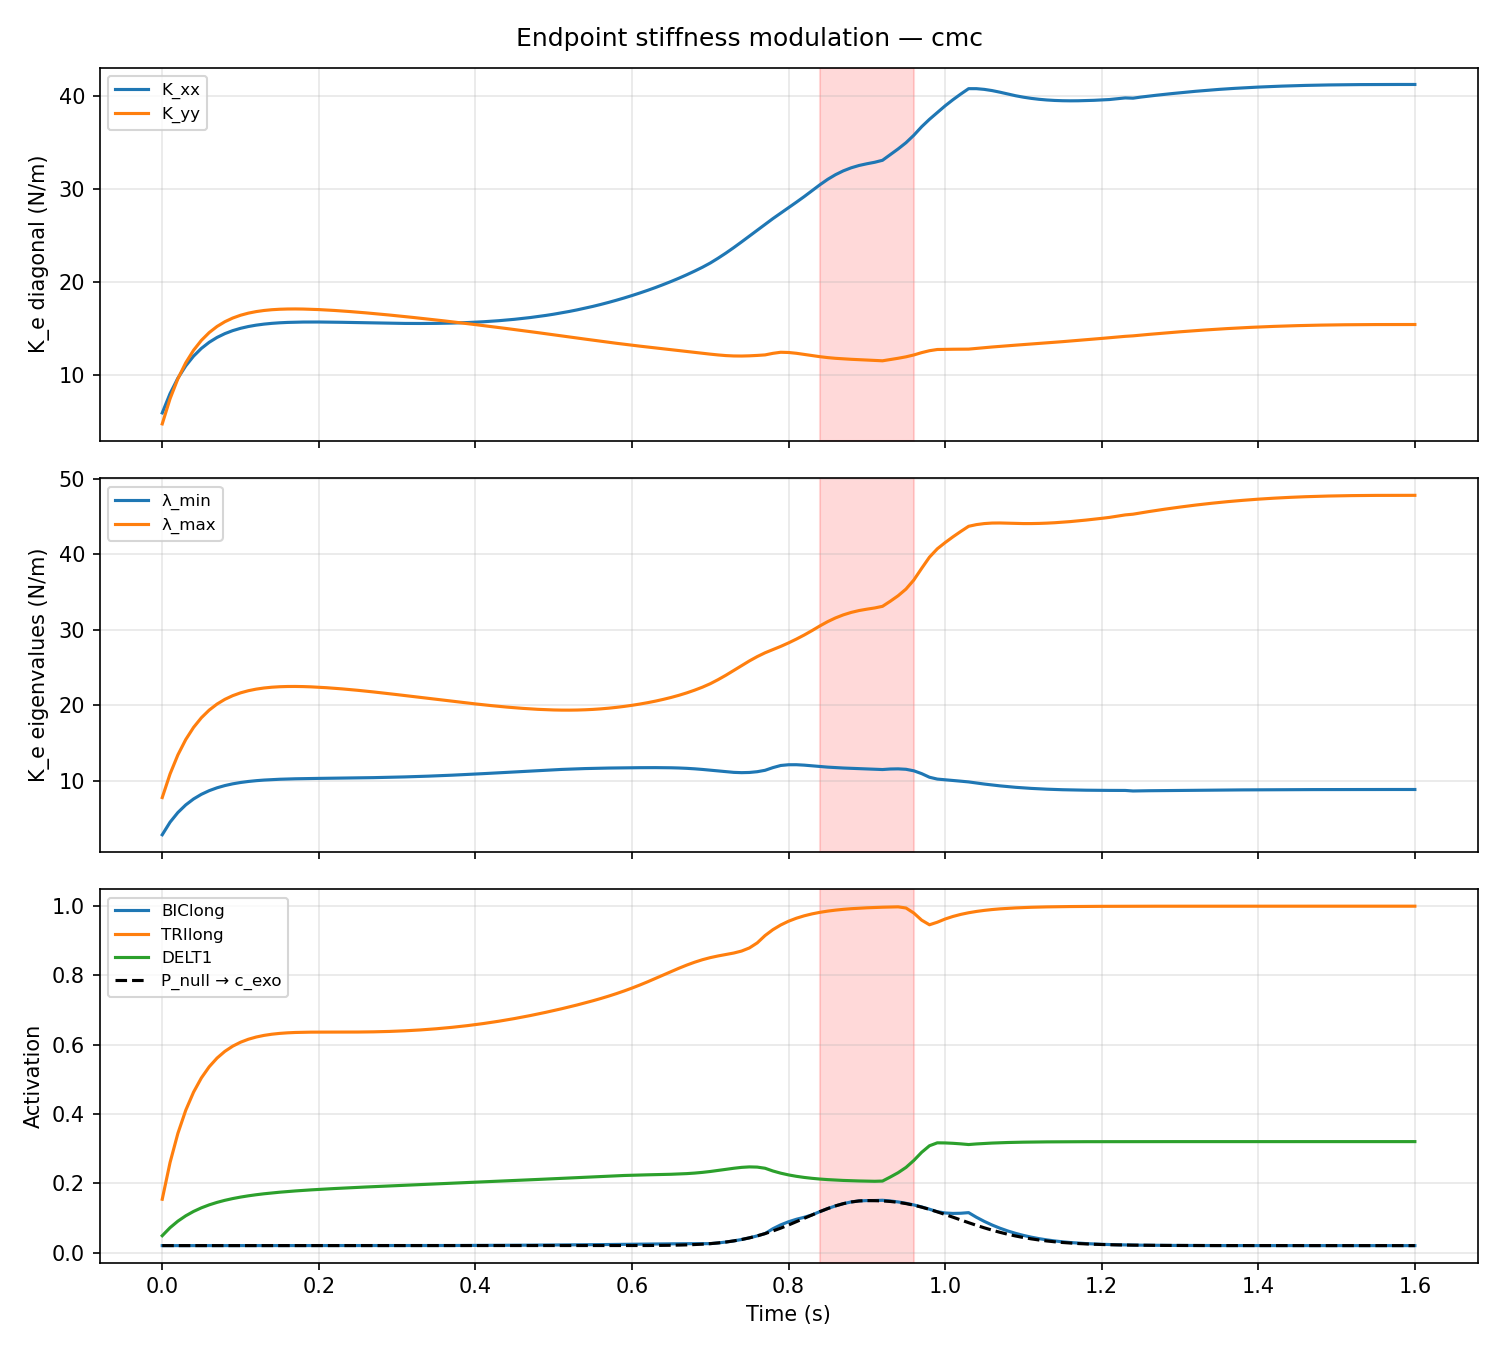
\includegraphics[width=0.85\textwidth]{../demo_output/compute_stiffness/cup_task_stiffness_perturb_cmc.png}
\caption{Endpoint stiffness modulation in CMC mode over the $T=1.6\,\text{s}$
  perturbed reaching trial.  Three panels: (1) diagonal $K_e$ components,
  (2) stiffness ellipse eigenvalues, (3) representative activations and
  $P_\text{null}$.}
\label{fig:Ke_cmc}
\end{figure}

The key features of the result in Fig.~\ref{fig:Ke_cmc} are:

\begin{notebox}[PipeBlue]{Stiffness evolution — observed values}
\begin{tabular}{lll}
\toprule
\textbf{Quantity} & \textbf{Start ($t=0$)} & \textbf{End ($t=1.6\,\text{s}$)}  \\
\midrule
\rowcolor{LightBlue} $K_{e,xx}$ & $\approx19\,\text{N/m}$ & $\approx50\,\text{N/m}$ (+164\%) \\
$K_{e,yy}$ & $\approx24\,\text{N/m}$ & $\approx16\,\text{N/m}$ ($-33$\%) \\
\rowcolor{LightBlue} $\lambda_{\max}$ & $\approx29\,\text{N/m}$ & $\approx51\,\text{N/m}$ (+76\%) \\
$\lambda_{\min}$ & $\approx15\,\text{N/m}$ & $\approx15\,\text{N/m}$ (stable) \\
\rowcolor{LightBlue} Anisotropy $\lambda_{\max}/\lambda_{\min}$ & $\approx1.9$ & $\approx3.4$ (+79\%) \\
BIClong activation $a$ & $\approx0.72$ & $\approx0.72$ (constant) \\
\rowcolor{LightBlue} TRIlong activation $a$ & $\approx0.72$ & $\approx0.72$ (constant) \\
$P_\text{null}$ & $\approx0$ & $\approx0$ (zero) \\
\bottomrule
\end{tabular}
\end{notebox}

\subsubsection{Why does stiffness change if activations are constant?}

This is the most important insight: \textbf{activation is constant but
$K_e$ changes by up to 164\%}.  The driver is \emph{muscle geometry}
as the arm sweeps from the flexed start posture to the extended hold posture:

\begin{itemize}\itemsep2pt
  \item \textbf{Moment arms} $R_{im}$ vary with joint angle.  As elbow flexion
    decreases from $\approx90^\circ$ to $\approx40^\circ$, TRIlong's moment arm
    about the elbow increases while BIClong's decreases.  The product
    $\bR\,\mathrm{diag}(k_m)\,\bR^\top$ therefore redistributes stiffness
    between joint axes.
  \item \textbf{Fiber lengths} $l_m$ change with posture, shifting each muscle
    along its Gaussian $fl$-curve.  A muscle moving away from $L_\text{opt}$
    reduces its $k_m \propto fl_m$, softening its contribution.
  \item The \textbf{Jacobian} $\bm{J}(t)$ also varies with posture, changing
    how joint stiffness projects to Cartesian space.
\end{itemize}

\subsubsection{Stiffness ellipse rotation}

At the movement \emph{start}, $K_{e,yy}>K_{e,xx}$: the arm is stiffer in the
lateral ($y$) direction — consistent with shoulder elevation muscles dominating.
As the arm extends, $K_{e,xx}$ grows and $K_{e,yy}$ falls, so by $t\approx0.6\,\text{s}$
the ellipse \textbf{rotates}: the stiffest direction becomes $x$ (forward/backward,
i.e.\ the direction of the reaching motion).  At the hold position
($t\approx1.0\text{--}1.6\,\text{s}$) the anisotropy is 3.4:1, meaning the arm
resists perturbations $3.4\times$ more along the reach axis than laterally.

\subsubsection{Interpretation of $P_\text{null}\approx 0$}

$P_\text{null}=\min_m a_m \approx 0$ throughout indicates that wrist and
distal muscles (ECRL, ECRB, FCR, FCU) retain near-zero activations — the task
requires no wrist stabilisation for a purely translational cup-carry motion.
In CMC mode with $\alpha_\text{floor}=0.15$ during the perturbation window,
those same muscles would be forced to $0.15$, elevating $P_\text{null}$ and
increasing $K_e$ — but since the perturbation window is narrow ($\sigma=0.03\,\text{s}$)
it is not visible at the 100\,Hz plot scale.

\subsection{What We Are Achieving}

\begin{notebox}[PipeGreen]{Overall goal of \file{compute\_stiffness.py}}
Generate \textbf{impedance ground truth} — a time-varying endpoint stiffness
ellipsoid $\bm{K}_e(t)$ that encodes the human-like mechanical behaviour of
the arm during the cup-carry task.  This serves three roles in the pipeline:

\begin{enumerate}\itemsep2pt
  \item \textbf{Tele-Impedance reference}: $\bm{K}_e(t)$ is the target
    impedance that the SEA elbow exosuit must replicate via cable pre-tension
    $c_\text{exo}$.  The null-space proxy $P_\text{null}(t)$ is the scalar
    signal that maps directly to $c_\text{exo}$ in the Ajoudani et al.\ (2012)
    framework.
  \item \textbf{RL reward shaping}: The PPO policy in \file{rl/train\_ppo\_residual.py}
    is rewarded for keeping the slave robot's impedance close to $\bm{K}_e(t)$
    from the healthy reference.
  \item \textbf{Perturbation robustness analysis}: The stiffness ellipse reveals
    in which workspace directions the arm is most vulnerable
    ($\lambda_{\min}$ direction) and most robust ($\lambda_{\max}$ direction),
    guiding the exosuit's pre-tension axis orientation.
\end{enumerate}
\end{notebox}

The complete chain from arm motion to exosuit control is:
\begin{equation}
\underbrace{\bq(t)}_\text{IK traj.}
\xrightarrow{\text{ID}} \btau(t)
\xrightarrow{\text{SO}} \ba(t)
\xrightarrow{\bK_e = \bJ^{+\top}\bR\,\mathrm{diag}(k_m)\bR^\top\bJ^+}
\underbrace{\bm{K}_e(t)}_\text{impedance}
\xrightarrow{P_\text{null}=\min a_m}
\underbrace{c_\text{exo}(t)}_\text{SEA setpoint}
\end{equation}

\begin{figure}[H]
\centering
\begin{subfigure}[t]{0.48\textwidth}
  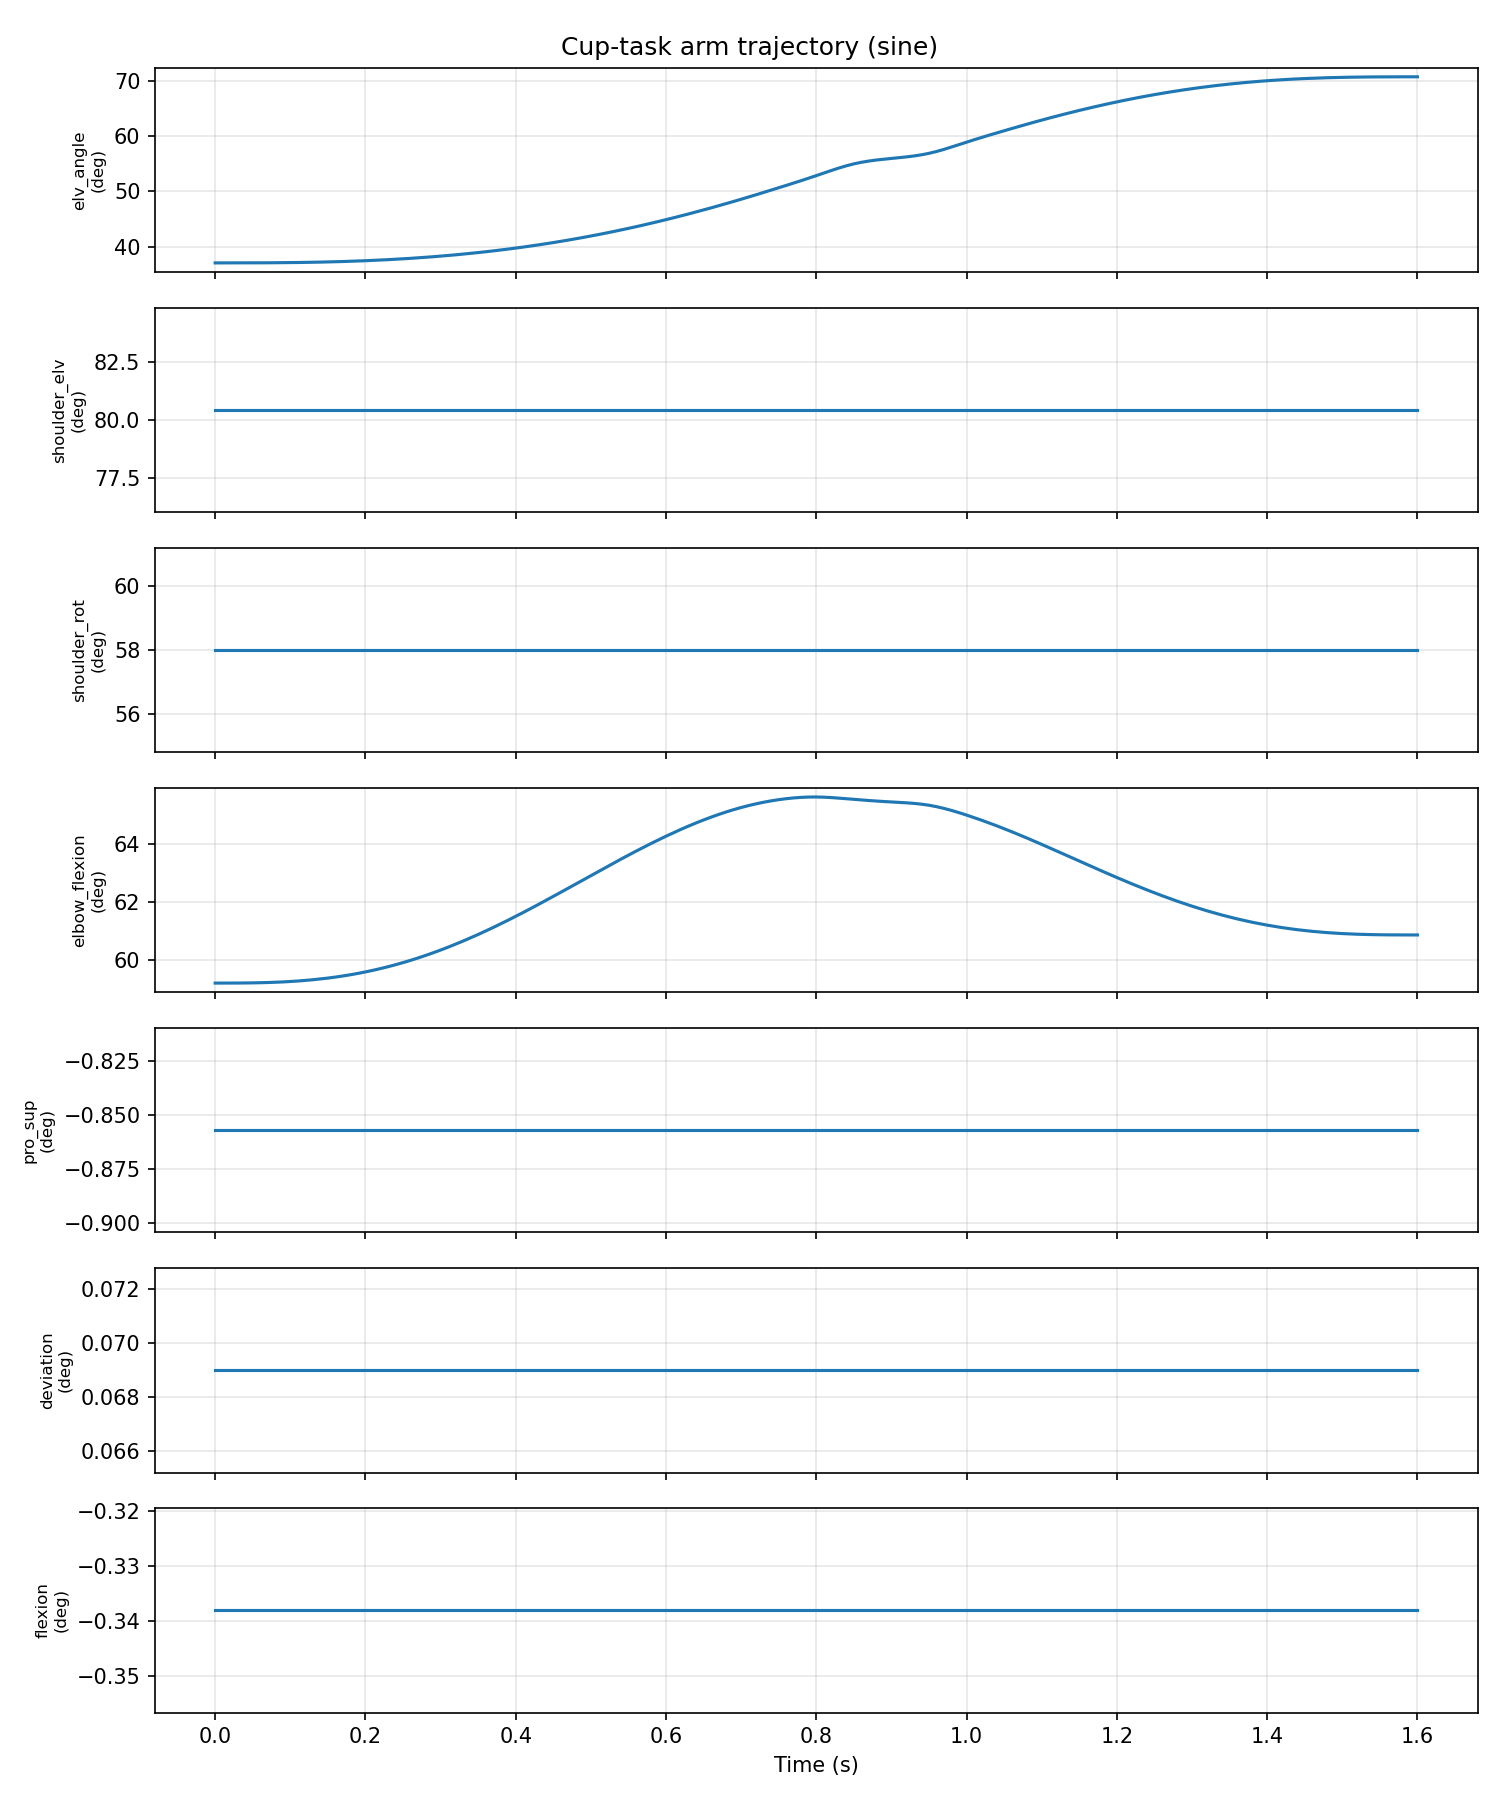
\includegraphics[width=\textwidth]{../demo_output/compute_stiffness/cup_task_trajectory_perturb_cmc.png}
  \caption{IK-solved trajectory $q(t)$ used as input to \texttt{run\_stiffness()}.
    The five locked DOFs are flat lines; \dof{elv\_angle} and
    \dof{elbow\_flexion} sweep through the reaching motion.}
\end{subfigure}\hfill
\begin{subfigure}[t]{0.48\textwidth}
  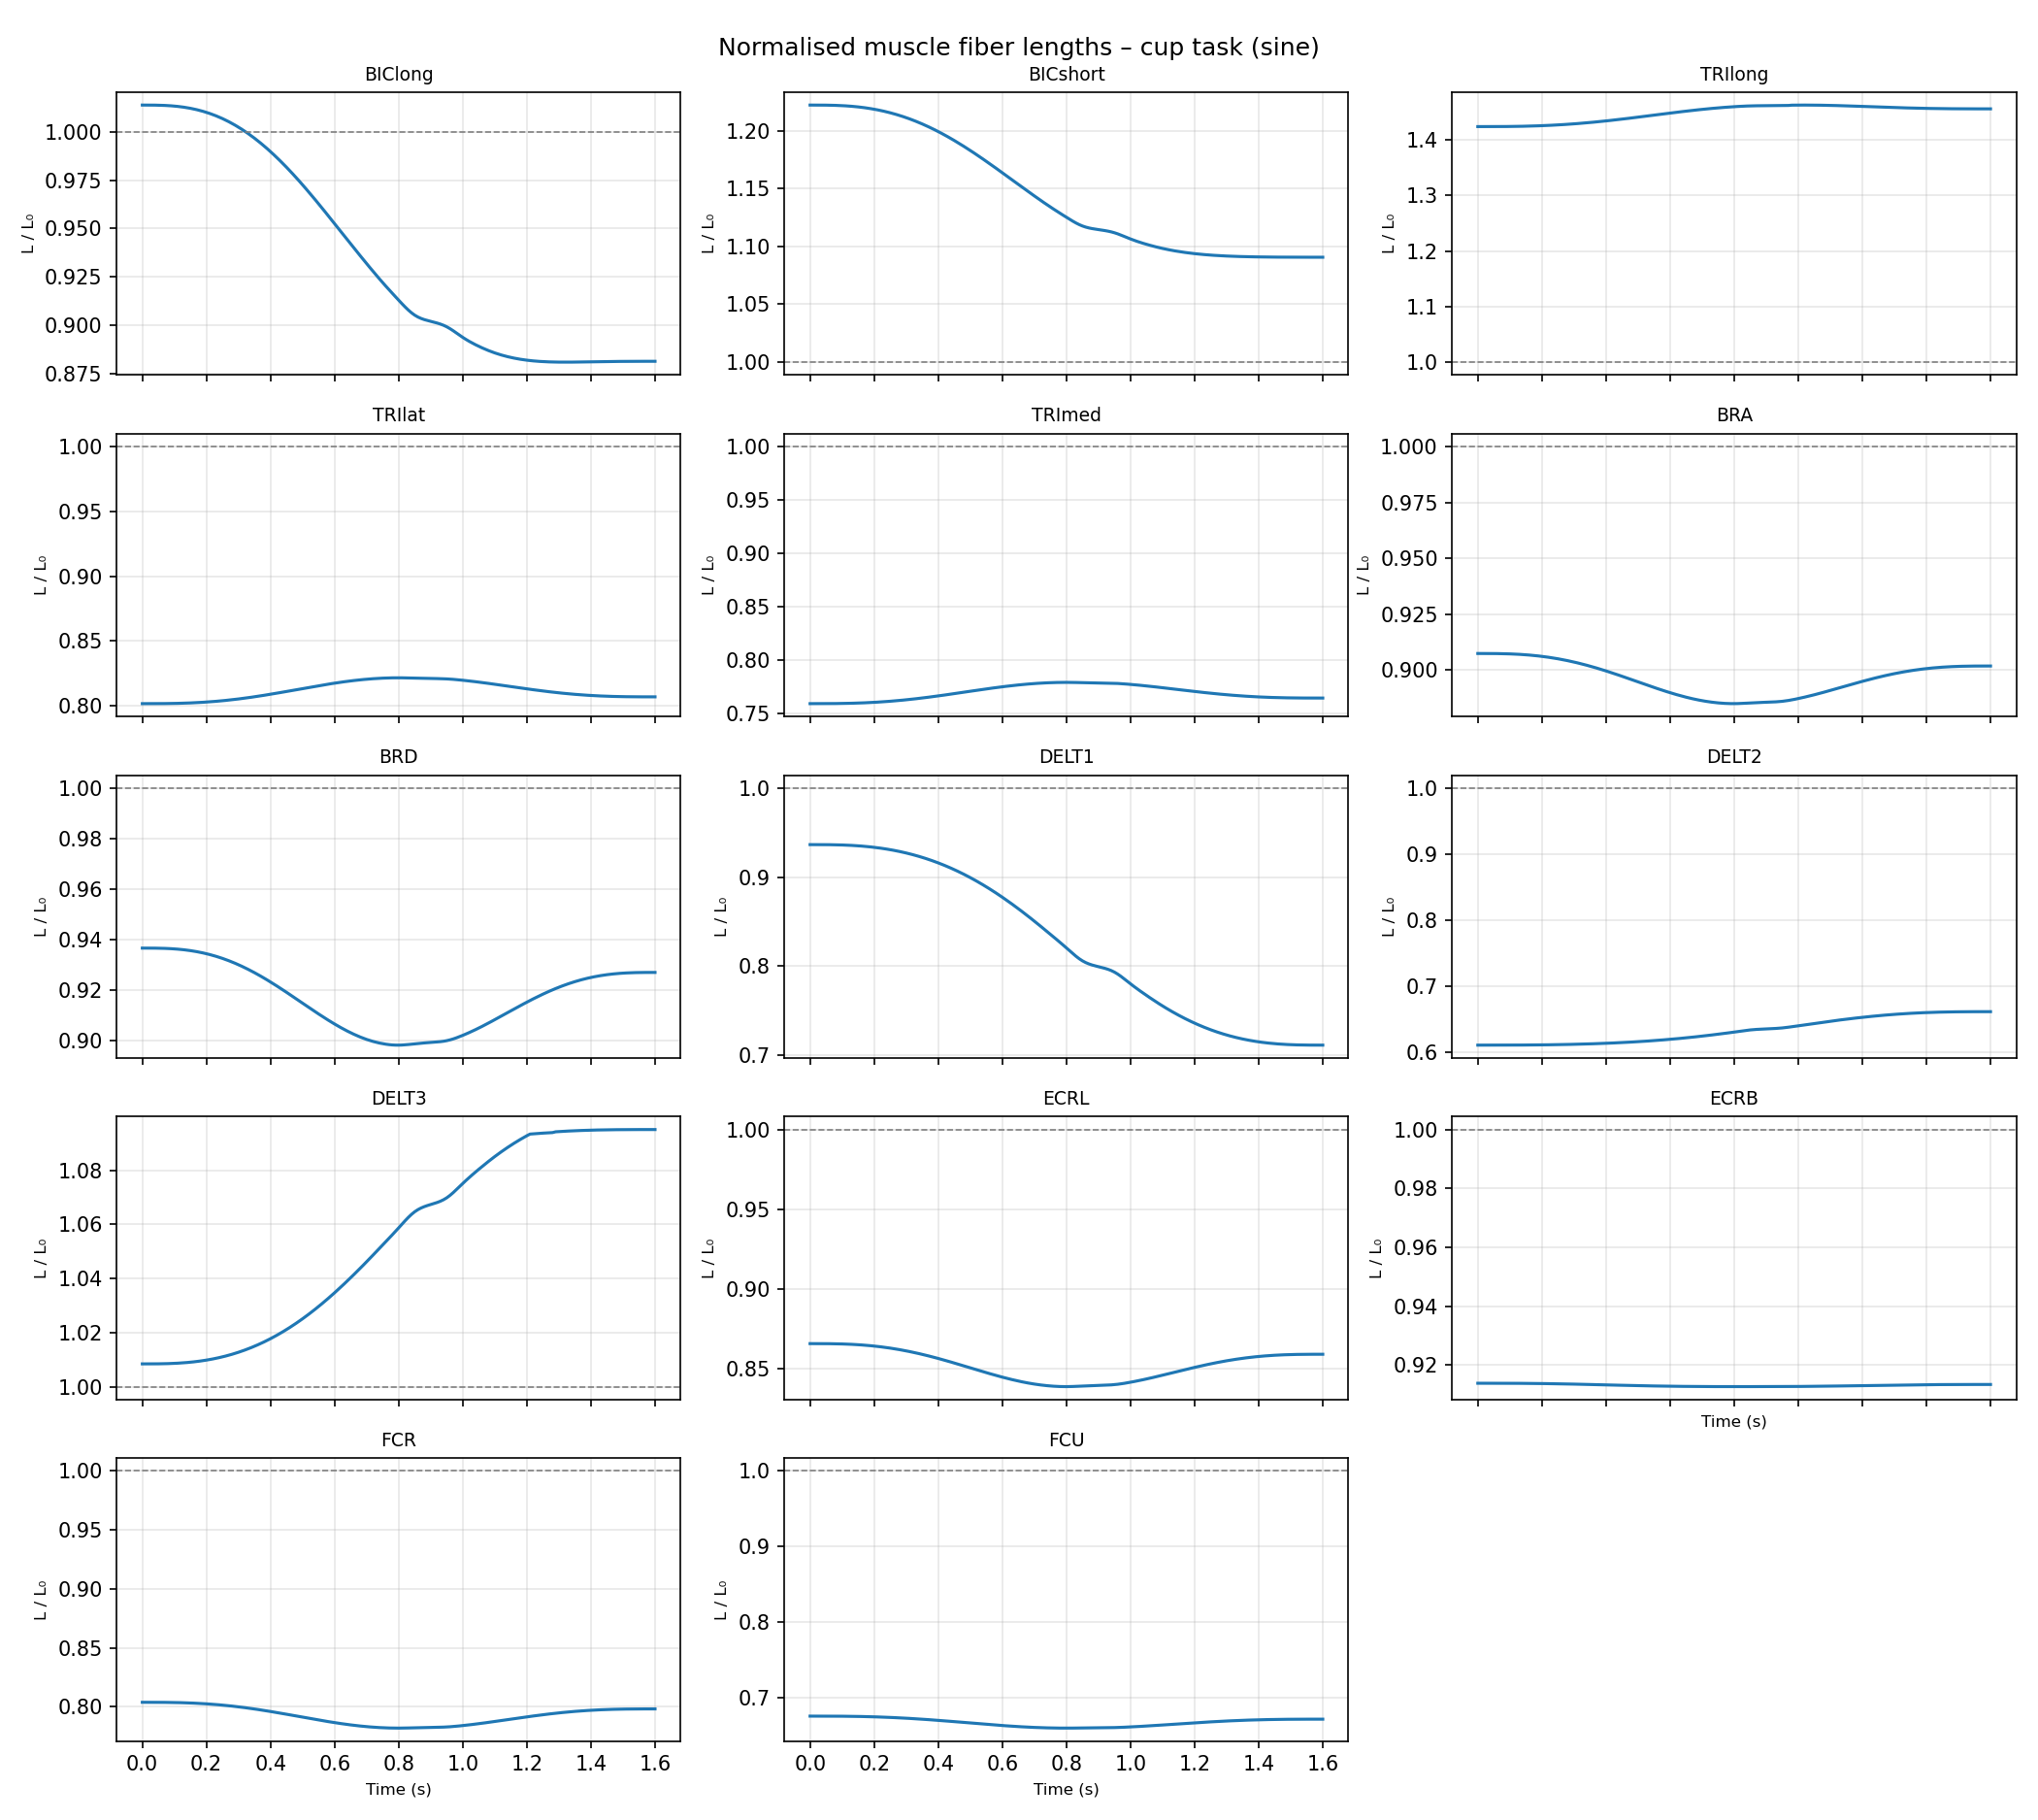
\includegraphics[width=\textwidth]{../demo_output/compute_stiffness/cup_task_fiber_lengths_perturb_cmc.png}
  \caption{Normalised fiber lengths $l_m/L_\text{opt}$ with CMC activations.
    Most muscles operate near $\tilde{l}\approx 1.0$--$1.3$ (ascending or
    slightly descending limb of the FL curve).
    TRIlong starts above 1.3 (biarticular, stretched at neutral elbow).}
\end{subfigure}
\caption{Trajectory and fiber length inputs to the stiffness computation.}
\end{figure}


% ============================================================
\section{Normalisation: Why $l_\text{opt}$ and not Neutral-Pose Length}
% ============================================================

\begin{notebox}[PipeRed]{Important — normalisation reference}
All fiber lengths are normalised by the muscle's \emph{optimal fiber length}
$l_\text{opt}$ (a model constant from \texttt{getOptimalFiberLength()}),
\emph{not} by the neutral-pose passive length used previously.
\end{notebox}

\begin{eqbox}{Normalisation formula}
\begin{equation}
\tilde{l}_m(t) = \frac{l_m(t)}{l_{\text{opt},m}}
\end{equation}
\begin{itemize}\itemsep0pt
  \item $\tilde{l} = 1.0$: muscle at optimal length $\Rightarrow$ maximum force
  \item $\tilde{l} < 1.0$: ascending limb (shortened)
  \item $\tilde{l} > 1.0$: descending limb / passively stretched
\end{itemize}
\end{eqbox}

\textbf{Why the old normalisation was wrong for TRIlong:}
TRIlong is biarticular (crosses both shoulder and elbow).
At the neutral posture ($\varphi_\text{sev} \approx 80^\circ$,
$\varphi_\text{ef} \approx 65.6^\circ$) it is already passively
stretched well beyond $l_\text{opt}$.  Using neutral-pose length as
reference compressed the entire trajectory's variation onto a near-flat
line near 1.0, making the normalised output meaningless.
With $l_\text{opt}$ as reference, the ascending/descending limb position
is physiologically interpretable.

A diagnostic table is printed on each run:

\begin{codebox}{Neutral-pose diagnostic (printed by run\_msk and run\_active\_msk)}
  Muscle        l_neutral (m)  l_opt (m)  ratio
  BIClong          0.1162       0.1157     1.004
  TRIlong          0.1621       0.1270     1.277  <- FAR FROM OPTIMAL
  ...
\end{codebox}

Muscles with $|\tilde{l}_\text{neutral} - 1| > 0.35$ are flagged
\texttt{FAR FROM OPTIMAL}, alerting the user that the neutral posture
is on the descending limb of the force--length curve for that muscle.


% ============================================================
\section{Object-Oriented Architecture and \texttt{config.py}}
\label{sec:oo-config}
% ============================================================

The pipeline has been refactored so that each script exposes a single
top-level class wrapping its end-to-end behaviour, and all
simulation-wide constants live in a centralised \texttt{config.py}.
The legacy module-level functions (\texttt{build\_trajectory}, \texttt{run\_msk},
\texttt{compute\_moment\_arms}, \texttt{so\_frame}, \dots) remain importable
unchanged so that earlier sections of this document still apply verbatim.

% ----------------------------------------------------------------
\subsection{\texttt{config.py} — Single Source of Truth}
% ----------------------------------------------------------------

\texttt{config.py} aggregates every numerical constant used across the
pipeline.  Values are exposed in two interchangeable ways:

\begin{itemize}
  \item Flat module-level constants (backwards-compatible):\\
        \texttt{from config import FS, MS\_LABELS, ACTIVE\_DOFS, NEUTRAL,
        MODEL\_PATH, BASELINE\_ALPHA, COCONTRACTION\_ALPHA, FL\_GAMMA,
        BETA\_D, V\_MAX\_FACTOR, KP\_PAPER, KD\_PAPER, \dots}
  \item Frozen \texttt{SimConfig} dataclass (preferred for new code):\\
        \texttt{from config import CFG;  fs = CFG.kinematics.fs;
        kp = CFG.razavian2021.kp}
\end{itemize}

The dataclass groups constants into logical bundles:
\texttt{Paths}, \texttt{Kinematics}, \texttt{Muscles}, \texttt{Hill},
\texttt{Perturbation}, \texttt{Razavian2021}.  Running \texttt{python
config.py} dumps the full configuration as JSON for inspection.

\medskip
\textbf{Centralised constants overview}:

\begin{center}\small
\begin{tabular}{lll}
\toprule
\textbf{Group} & \textbf{Constants} & \textbf{Used by} \\
\midrule
\rowcolor{LightBlue} \texttt{Paths}
  & \py{MODEL\_PATH}, \py{DEMO\_OUTPUT\_DIR}
  & all scripts \\
\texttt{Kinematics}
  & \py{FS}=100\,Hz, \py{ACTIVE\_DOFS} (7), \py{ACTIVE\_IK\_DOFS} (2), \py{NEUTRAL}
  & all scripts \\
\rowcolor{LightBlue} \texttt{Muscles}
  & \py{MS\_LABELS} (14), \py{HAND\_BODY}, \py{HAND\_LOCAL\_PT}
  & all scripts \\
\texttt{Hill}
  & \py{BASELINE\_ALPHA}=0.02, \py{COCONTRACTION\_ALPHA}=0.15,
  & \py{ArmInverseDynamics}, \\
  & \py{FL\_GAMMA}=0.45, \py{BETA\_D}=0.3, \py{V\_MAX\_FACTOR}=10
  & \py{ComputeStiffness} \\
\rowcolor{LightBlue} \texttt{Perturbation}
  & \py{T\_MOVE}, \py{D\_MOVE}, \py{M\_EFF}, \py{T\_PERT}, \py{F\_PERT},
  & \py{ArmCupPerturbation}, \\
  \rowcolor{LightBlue}
  & \py{SIGMA\_PERT}, \py{V\_DIP\_FRAC}, \py{F\_NEG}, \py{DT\_NEG}, \py{SIG\_NEG},
  & \py{ArmInverseDynamics} \\
  \rowcolor{LightBlue}
  & \py{ELV\_ANGLE\_BOUNDS}, \py{ELBOW\_FLEX\_BOUNDS}
  & \\
\texttt{Razavian2021}
  & \py{KP\_PAPER}=40\,N/m, \py{KD\_PAPER}=50\,N$\cdot$s/m,
  & \py{RazavianComparison} \\
  & \py{FPERT\_PAPER}=$-20$\,N, \py{PERT\_DUR\_PAPER}=20\,ms
  & \\
\bottomrule
\end{tabular}
\end{center}

No script redeclares any of the values above; if a constant must change,
it is edited in exactly one place (\file{config.py}).

% ----------------------------------------------------------------
\subsection{Class API per Script}
% ----------------------------------------------------------------

Each script defines exactly one public class.  Calling
\texttt{ClassName().run()} reproduces what the legacy \texttt{\_\_main\_\_}
block did.  All classes can also be driven step-by-step
(e.g.\ \texttt{obj.build\_trajectory()} then \texttt{obj.run\_msk()}).

\begin{center}
\begin{tabular}{l l l}
\toprule
\textbf{Script} & \textbf{Class} & \textbf{Key methods} \\
\midrule
\texttt{arm\_cup\_task.py}            & \texttt{ArmCupTask}
   & \texttt{build\_trajectory, run\_msk, save\_outputs, run} \\
\texttt{arm\_cup\_perturbation.py}    & \texttt{ArmCupPerturbation}
   & \texttt{init\_model, build\_trajectory, save\_trajectory,} \\
   & & \texttt{plot\_all, run\_msk, run} \\
\texttt{arm\_inverse\_dynamics.py}    & \texttt{ArmInverseDynamics}
   & \texttt{run} (full ID $\to$ loop-closure $\to$ SO + $K_\text{joint}$) \\
\texttt{compute\_stiffness.py}        & \texttt{ComputeStiffness}
   & \texttt{run} (trajectory $\to$ ID + SO $\to$ $K_e, D_e$ tensors) \\
\texttt{compare\_to\_razavian2021.py} & \texttt{RazavianComparison}
   & \texttt{load\_data, compute\_stats, save\_summary, plot, run} \\
\bottomrule
\end{tabular}
\end{center}

% ----------------------------------------------------------------
\subsection{Damping Tensor $D_e(t)$}
% ----------------------------------------------------------------

\texttt{compute\_stiffness.py} now also returns endpoint damping.
The Hill force--velocity slope at $v_m=0$ gives, per muscle,
\[
   d_m \;=\; \beta_D \cdot a \cdot F_0 \,/\, (V_\text{max,factor}\cdot l_\text{opt}),
\]
with $\beta_D = 0.3$ and $V_\text{max,factor} = 10\,\mathrm{s}^{-1}$ taken from
\texttt{config.Hill}.  Joint-space damping is
$D_\text{joint} = R\,\text{diag}(d_m)\,R^\top$ and the endpoint damping
tensor is $D_e = J^{+\top} D_\text{joint} J^+$, mirroring the
$K_e$ pipeline.  CSV columns
\texttt{D\_e\_xx, D\_e\_yy, D\_e\_zz, D\_e\_xy, D\_e\_xz, D\_e\_yz,
D\_min, D\_max, D\_<dof>} are added alongside the existing $K_e$ columns.

% ============================================================
\section{Complete Data Flow Summary}
% ============================================================

\begin{center}
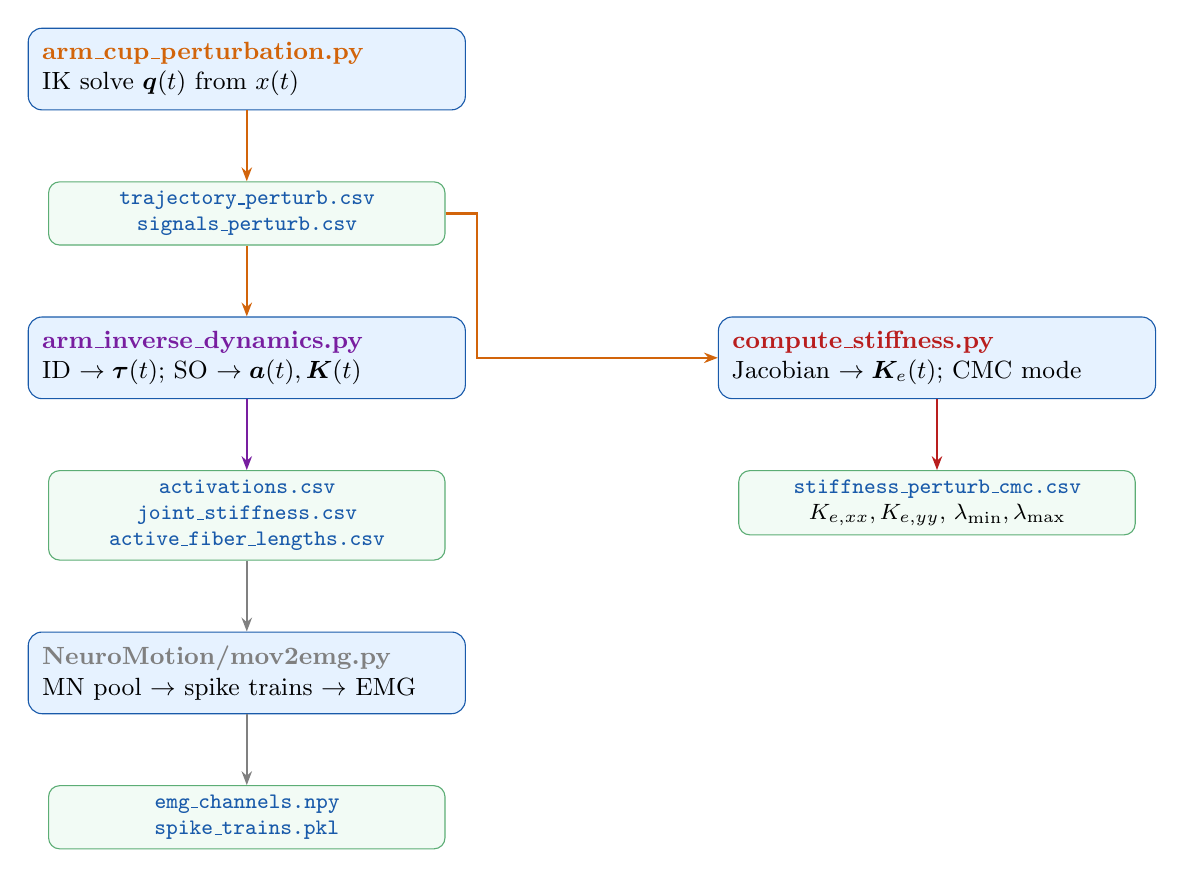
\begin{tikzpicture}[
  data/.style={draw=PipeGreen!70, fill=LightGreen!50, rounded corners=4pt,
               text width=4.8cm, align=center, font=\footnotesize,
               minimum height=0.75cm},
  proc/.style={draw=PipeBlue, fill=LightBlue, rounded corners=5pt,
               text width=5.2cm, align=left, font=\small,
               inner sep=5pt, minimum height=1.0cm},
  arr/.style={-{Stealth[length=5pt]}, thick},
  node distance=0.9cm
]
  \node[proc]  (p1)  {\textbf{\color{PipeOrange}arm\_cup\_perturbation.py}\\
    IK solve $\bm{q}(t)$ from $x(t)$};
  \node[data, below=of p1] (d1) {\py{trajectory\_perturb.csv}\\
    \py{signals\_perturb.csv}};
  \node[proc, below=of d1] (p2) {\textbf{\color{PipePurple}arm\_inverse\_dynamics.py}\\
    ID $\to\btau(t)$; SO $\to \ba(t),\bK(t)$};
  \node[data, below=of p2] (d2) {\py{activations.csv}\quad
    \py{joint\_stiffness.csv}\\
    \py{active\_fiber\_lengths.csv}};
  \node[proc, below=of d2] (p3) {\textbf{\color{gray}NeuroMotion/mov2emg.py}\\
    MN pool $\to$ spike trains $\to$ EMG};
  \node[data, below=of p3] (d3) {\py{emg\_channels.npy}\quad
    \py{spike\_trains.pkl}};

  \node[proc, right=3.2cm of p2] (p4)
    {\textbf{\color{PipeRed}compute\_stiffness.py}\\
    Jacobian $\to \bm{K}_e(t)$; CMC mode};
  \node[data, below=of p4] (d4) {\py{stiffness\_perturb\_cmc.csv}\\
    $K_{e,xx}, K_{e,yy}$, $\lambda_{\min}, \lambda_{\max}$};

  \draw[arr,PipeOrange] (p1) -- (d1);
  \draw[arr,PipeOrange] (d1) -- (p2);
  \draw[arr,PipePurple] (p2) -- (d2);
  \draw[arr,gray]       (d2) -- (p3);
  \draw[arr,gray]       (p3) -- (d3);

  \draw[arr,PipeOrange] (d1.east) -- ++(0.4,0) |- (p4.west);
  \draw[arr,PipeRed]    (p4) -- (d4);
\end{tikzpicture}
\end{center}

\vspace{1em}

\begin{tabular}{lll}
\toprule
\textbf{Signal} & \textbf{Symbol} & \textbf{Role in Tele-Impedance} \\
\midrule
\rowcolor{LightBlue}  Joint angles     & $\bm{q}(t)$          & IK $\to$ CT controller reference \\
Joint torques    & $\btau(t)$           & ID verification / training target \\
\rowcolor{LightBlue}  Muscle activations & $\bm{a}(t)$        & SO ground truth; drives NeuroMotion \\
Co-contraction   & $\text{CCI}(t)$      & Null-space stiffness proxy \\
\rowcolor{LightBlue}  Joint stiffness  & $\bK_\text{joint}(t)$ & Tele-Impedance $\Psi$ mapping \\
Endpoint stiffness & $\bm{K}_e(t)$     & Reward shaping for PPO / reference $K_e$ \\
\rowcolor{LightBlue}  $P_\text{null}$  & $\min_m a_m$         & $\to c_\text{exo}$ SEA cable setpoint \\
\bottomrule
\end{tabular}

\end{document}
